\chapter{Results}
\label{ch:results}
	\section{Proximate deforestation drivers}
	\label{sec:results_deforestation}
		\subsection{Forest definition}
		\label{subsec:results_forest_definition}
			By applying the approach described in section \ref{subsubsec:forest_definition} our goal is to determine at which canopy density the agreement between the \ac{GL30} an the \ac{GFC} dataset is at its maximum. This process should ensure that we keep the largest number of tree cover loss samples from the \ac{GFC} dataset, while harmonizing the tree cover definition between both layers. For the entire study extent our hypothesis is, that the tree cover agreement is at its maximum within the canopy density interval of $(30,100]$. For Latin America and Asia/Australia we assumed, that the best results could be achieved within the same canopy density threshold. For Africa we assumed that the maximum agreement could be observed within the interval of $(10,100]$ because this region comprises a large area of sparse woodland cover. The following paragraphs present our results for the three regions in the following order: Latin America, Asia/Australia and Africa. The last paragraph discusses the results on global scale and deduces which canopy density threshold we used for our mapping of \acp{PDD}.
			\begin{figure}[ht]
				\centering
				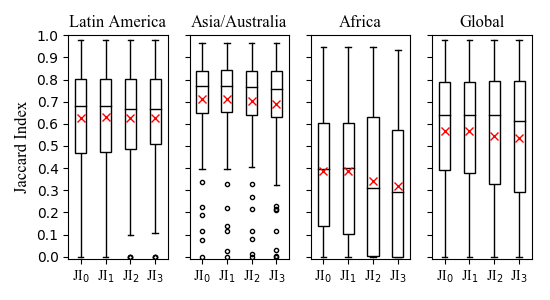
\includegraphics[scale=.91]{img/jaccard}
				\caption[Tree cover similarity distribution]{\textbf{Tree cover similarity distribution:} This box-plot shows the distribution of Jaccard Index (JI) for each raster image tile pair of GlobeLand30 and Global Forest Change tree cover from 2000. The labels $JI_0$, $JI_1$, $JI_2$, and $JI_3$ on the x-axis account for the canopy density classes $(0,100]$, $(10,100]$, $(20,100]$, and $(30,100]$, respectively. The y-axis is the Jaccard Index of the corresponding raster image pair, where 0 is a total disagreement and 1 a total agreement. Red crosses within the $Q_{25}$, $Q_{50}$, and $Q_{75}$ boxes highlight the sample mean. Whiskers are 1.5 times the inter-quartile range (IQR).}
				\label{fig:jaccard}
			\end{figure}

			For Latin America figure \ref{fig:jaccard} shows the \acp{JI} distribution for our experiment groups. Within the four canopy density experiments the sample mean does not change significantly. It is approximately 0.62, while the sample median decreases from 0.68 to 0.66 from the first experiment group to the last. The upper 25\% of the first experiment interval has a tree cover similarity ranging between approximately 0.8 and 1. The figure \ref{fig:jaccard_americas_appendix} in the appendix \ref{ch:appendix} suggests that exclusions of canopy densities smaller than 11\% increases slightly the tree cover agreement of the upper 25\%, but the exclusion of higher canopy density provides no further benefit. This can be explained by the fact that the upper percentile already contains samples with a high tree cover agreement and it is to assume that only a small number of pixels have canopy density smaller than 30\%. Therefore, the interval change has only a small impact on these samples. The figure \ref{fig:jaccard_americas_appendix} reveals a strong regional dependency of tree cover agreement within the different canopy density classes of the lower percentiles. The samples from the northern hemisphere show a decline in agreement, while the samples of the southern hemisphere show a increase of agreement. The strong up-shift of the southern samples within the last two experiment groups increases the quartile range of lower percentile. In general, this suggests that samples with low tree cover agreement benefit by the exclusion of lower canopy densities. No general trend is observable for the mobility of the samples within the $Q_1$ and $Q_3$ percentile. For the first two experiments the quartile range is between 0.5 and 0.8. For the last two experiment groups the inter-quartile range declines slightly. This suggests that tiles within this quartile could benefit from a local optimization of canopy density exclusion.

			We applied a Wilcoxon signed-rank test to deduce which canopy density class yields the highest tree cover agreement overall samples in Latin America. Table \ref{tab:wilcoxontwosided_regions} shows the results for the two-sided test and table \ref{tab:wilcoxontwosided_regions} for the one-sided test. The two-sided test reveals that only the similarity distribution between the experiment groups $JI_0$ and $JI_1$ is significantly different ($p<0.01$), while the comparison of the other distributions suggest that they are equal. The directional test of $JI_0$ and $JI_1$ suggests that the regional tree cover agreement is significantly greater ($p<0.005$) if canopy densities smaller than 10\% are excluded. The directional test does not confirm that the distribution if $JI_1$ is significantly greater than $JI_2$ and $JI_3$. Therefore it can be assumed that the exclusion of lower canopy densities could yield better results for certain tiles. For Latin America the results of our experiment suggests that the tree cover agreement between the \ac{GL30} stratum and \ac{GFC} stratum is at its maximum for canopy densities greater than 10\%. In case of local studies or for a smaller scale the canopy density should be selected by a single tile approach to optimize the tree cover agreement by maximizing the number of data points from the \ac{GFC} dataset.
			\begin{table}[ht]
				\centering
				\caption[Continental experiment group comparison]{\textbf{Continental experiment group comparison:} This table shows the results of a two-sided Wilcoxon signed-rank test to detect continental differences in the tree cover agreement by considering different canopy densities between GlobeLand30 and Global Forest Change 2000. The classes $JI_0$, $JI_1$, $JI_2$, and $JI_3$ as row and column headings account for the canopy density classes (0,100], (10,100], (20,100], and (30,100], respectively. The test hypothesis is H$_0$: $X_1=X_2$ where $X_1$ is the column $JI_n$ class and $X_2$ the row $JI_n$ class. The significance is indicated by $p^{*}<0.05$, $p^{**}<0.02$, and $p^{***}<0.01$.}
				\label{tab:wilcoxontwosided_regions}
				\begin{tabular}{llllllllllll}
					\hline
					& \multicolumn{3}{c}{Latin America} && \multicolumn{3}{c}{Asia/Australia} && \multicolumn{3}{c}{Africa} \\\cline{2-4}\cline{6-8}\cline{10-12}
					Cls & JI$_0$ & JI$_1$ & JI$_2$ && JI$_0$ & JI$_1$ & JI$_2$ && JI$_0$ & JI$_1$ & JI$_2$ \\\hline
					JI$_1$ & .00$^{***}$ & - & - && .71 & - & - && .22 & - & - \\
					JI$_2$ & .30 & 1. & - && .00$^{***}$ & .00$^{***}$ & - && .09 & .09  & - \\
					JI$_3$ & .64 & 1. & 1. && .00$^{***}$ & .00$^{***}$ & .00$^{***}$ && .00$^{***}$ & .00$^{***}$ & .00$^{***}$ \\\hline
				\end{tabular}
			\end{table}
			\begin{table}[ht]
				\centering
				\caption[Continental experiment group directional comparison]{\textbf{Continental experiment group directional comparison:} This table shows the results of a one-sided Wilcoxon signed-rank test to detect the direction of continental differences in the tree cover agreement by considering different canopy densities between GlobeLand30 and Global Forest Change 2000. The classes $JI_0$, $JI_1$, $JI_2$, and $JI_3$ as row and column headings account for the canopy density classes (0,100], (10,100], (20,100], and (30,100], respectively. The test hypothesis is H$_0$: $X_1\leq X_2$ and H$_0$: $X_2\geq X_1$ where $X_1$ is the column $JI_n$ class and $X_2$ the row $JI_n$ class. The significance is indicated by $p^{*}<0.05$, $p^{**}<0.025$, $p^{***}<0.01$, and $p^{\dagger}<0.005$.}
				\label{tab:wilcoxononesided_regions}
				\begin{tabular}{lllllllllllllll}
					\hline
					& \multicolumn{4}{c}{Latin America} && \multicolumn{4}{c}{Asia/Australia} && \multicolumn{4}{c}{Africa} \\\cline{2-5}\cline{7-10}\cline{12-15}
					Cls & JI$_0$ & JI$_1$ & JI$_2$ & JI$_3$ && JI$_0$ & JI$_1$ & JI$_2$ & JI$_3$ && JI$_0$ & JI$_1$ & JI$_2$ & JI$_3$ \\\hline
					JI$_0$ & - & .00$^{\dagger}$ & .14 & .33 && - & 1. & 1. & 1. && - & .65 & 1. & 1. \\
					JI$_1$ & 1. & - & .55 & .55 && .36 & - & 1. & 1. && .89 & - & 1. & 1. \\
					JI$_2$ & 1. & 1. & - & .55 && .00$^{\dagger}$ & .00$^{\dagger}$ & - & 1. && .03$^{*}$ & .03$^{*}$ & - & 1. \\
					JI$_3$ & 1. & 1. & 1. & - && .00$^{\dagger}$ & .00$^{\dagger}$ & .00$^{\dagger}$ & - && .00$^{\dagger}$ & .00$^{\dagger}$ & .00$^{\dagger}$ & - \\\hline
				\end{tabular}
			\end{table}

			Asia/Australia present a \ac{JI} mean of 0.7 as figure \ref{fig:jaccard} suggest. The sample mean decreases slightly at higher canopy density intervals. Further, the median is approximately 0.8, and shows a slight decrease at higher canopy density intervals. For all experiment groups the range of the upper percentiles is between approximately 0.85 and 0.96, while the maximum agreement decreases slightly. Figure \ref{fig:jaccard_asia_appendix} in the appendix \ref{ch:appendix} reveals that in general the tree cover agreement increases if canopy densities below 10\% are excluded, but the exclusion of canopy densities above 20\% reverts this. For Asia/Australia the lower percentile ranges between approximately 0 and 0.65, while most of the samples show a decline in tree cover agreement if canopy densities above 20\% are excluded. Within the $Q_{1,3}$ percentile a per tile relationship is observable. The range of this percentile is between 0.65 and 0.85 for the first two experiment groups $JI_0$ and $JI_1$, while the range increases for the last two experiment groups. As mentioned no clear trend is observable some of the samples benefit if the considered canopy density interval is lift above 30\% and some show a decrease in agreement if the canopy density is lift over 10\%. 

			The two-sided Wilcoxon test in table \ref{tab:wilcoxontwosided_regions} reveals that the similarity distribution is significantly different ($p<0.01$) between each experiment group except for the experiment group pair of $JI_1$ and $JI_0$. The directional test in table \ref{tab:wilcoxononesided_regions} reveals, that the tree cover agreement distributions of $JI_2$ and $JI_3$ are significantly smaller than $JI_0$ and $JI_1$ ($p<0.005$). These results show that the distributions of $JI_0$ and $JI_1$ have no directional differences. This could be explained by a regional or tile-wise agreement component. While some of the tiles show strong increase in similarity if canopy density is set to 10\%, others show a decrease. A more detailed analysis could be performed by applying a smaller canopy density step-size. For studies targeting the region Asia/Australia the results of the directional tests suggest to use all data from the \ac{GFC} stratum within the canopy density interval of $(0,100]$. While the figure \ref{fig:jaccard_asia_appendix} suggests to include all data from the interval $(10,100]$.

			For Africa the box-plot in figure \ref{fig:jaccard} shows that the similarity quartile range of the upper 75\% is the greatest among our study regions. It ranges between 0.15 and 1.0 for $JI_0$, while the range increases if smaller canopy densities are excluded. The first two experiment groups $JI_0$ and $JI_1$ have a nearly similar mean and median of approximately 0.38 and 0.4, respectively. Whereas both metrics show a strong decline to 0.33 and 0.3 in the last two experiment groups $JI_2$ and $JI_3$, respectively. Figure \ref{fig:jaccard_africa_appendix} in the appendix \ref{ch:appendix} reveals that the upper 25\% does not benefit by the exclusion of smaller canopy densities. This behavior is largely different to Latin America and Asia/Australia. Africa has the greatest number of tiles where the tree cover agreement is smaller than 0.1. For the second experiment group ($JI_1$) 11 tiles from the \ac{AISM} have a complete disagreement ($JI=0$) if the canopy density interval is reduced to $(10,100]$. This trend continues if the canopy density interval is further reduced. This already suggests that reducing the canopy density interval for Africa is not feasible. 

			The two-sided test in table \ref{tab:wilcoxontwosided_regions} reveals that $JI_3$ is significantly different ($p<0.01$) in its similarity distribution compared to the other experiment groups $JI_0$, $JI_1$, and $JI_2$, respectively. The other experiment groups could origin from the same similarity distribution. Especially, the tree cover agreement between $JI_0$ and $JI_1$ shows strong evidences that it could originate from the same distribution. This is comparable with the Asia/Australian continental region. For Africa the table \ref{tab:wilcoxononesided_regions} shows the directional component of the tree cover agreement between the experiments groups. The tree cover agreement of the two experiment groups $JI_2$ and $JI_3$ is significantly smaller than $JI_0$ or $JI_1$ as the table suggest. Therefore, the exclusion of canopy densities above 10\% reduces the continental tree cover agreement in Africa. For the first two experiment groups $JI_0$ and $JI_1$ no directional agreement component could be proofed, but the figure \ref{fig:jaccard_africa_appendix} shows a strong regional component of tree cover agreement. The strong regional component can be explained by the high share of sparse woodland in Africa. The figure \ref{fig:africa_tree_cover} in section \ref{subsec:results_tree_cover_and_deforestation} shows that different from Asia/Australia and Latin America a vast amount of African tree cover has a canopy density between 0\% and 46\%. The results for Africa suggests to set the canopy density interval to $(0,100]$ to optimize the tree cover agreement between the \ac{GL30} stratum and \ac{GFC} stratum on a continental level.

			The table \ref{tab:wilcoxononesided_comparison} in the appendix \ref{ch:appendix} shows that in Asia/Australia the tree cover similarity between the \ac{GL30} stratum and \ac{GFC} stratum is the greatest out of all three regions. Only within the last experiment group ($JI_3$) the median tree cover agreement between Asia/Australia and Latin America could be the same as shown in table \ref{tab:wilcoxontwosided_comparison}. Africa has the poorest tree cover agreement out of our three continental regions. Asia's higher tree cover agreement compared to Latin America could relate to the smaller total landmass and the high quantity of dense forest cover. Therefore both global \ac{LC} datasets have a smaller chance to miss forest covered pixels. That both regions achieve better tree cover similarity than Africa could be explained by the high amount of dense forest cover within these continental regions. From our results we hypothesize that the probability of misclassification of forest cover increases the lower the canopy density is. In regards of tile-wise tree cover agreement optimization Africa would  benefit the most out of the three regions. In Asia/Australia and Latin America only certain tiles would benefit from a exclusive optimization as the figures \ref{fig:jaccard_americas_appendix} and \ref{fig:jaccard_asia_appendix} suggests.

			On the far right of figure \ref{fig:jaccard} the tree cover agreement of the entire study extent is shown. The sample mean and median differ between the first two experiment groups and the last two groups. For the first two groups the mean and median account for 0.56 and 0.63, respectively. The last two experiment groups show a decline to 0.53 and 0.53 for mean and median. For the upper percentile the same statement as for the regions holds true. In general, the samples with high tree cover agreement benefit from the exclusion of lower canopy densities. The lower percentile shows strong regional or tile-wise tree cover agreement dependencies. If we consider the entire sample range the mid percentile steadily increases its quartile range. As mentioned in the regional analysis, this percentile is characterized by inhomogeneous changes of tree cover agreement by the step-wise change of the canopy density. In general the trend points downwards as the decrease in median and the quartile range increase show. 

			The results of the two-sided Wilcoxon test in table \ref{tab:wilcoxontwosided_all} show a significant difference in distribution (p<0.02 and p<0.01) between each experiment group except for the groups $JI_0$ and $JI_2$ where the similarity distribution could be originated from the same distribution. Table \ref{tab:wilcoxononesided_all} highlights the directional component of these distributional differences. At a global scale the tree cover agreement is at its maximum if we set the canopy density interval to $(10,100]$. The second experiment group $JI_1$ is significantly greater than $JI_0$ (p<0.005) and the last two groups $JI_2$ and $JI_3$ are significantly smaller (p>0.005) than $JI_1$. Further, the tree cover agreement of $JI_0$ is significantly greater than (p<0.005 and p<0.05) $JI_2$ and $JI_3$. Therefore it is proved, that canopy densities above 20\% reduce the tree cover agreement between \ac{GL30} and \ac{GFC} on a global level. On a global scale as the analysis on tree cover agreement suggests the maximum similarity can be achieved within the $JI_1$ interval. Therefore we decided to proceed for our study of \acp{PDD} and the derived products with this definition of tree cover.
			\begin{table}[ht]
				\centering
				\caption[Global experiment group comparison]{\textbf{Global experiment group comparison:} This table shows a two-sided Wilcoxon signed-rank test to detect differences in the tree cover agreement by considering different canopy densities between GlobeLand30 and Global Forest Change 2000. The classes $JI_0$, $JI_1$, $JI_2$, and $JI_3$ as row and column headings account for the canopy density classes (0,100], (10,100], (20,100], and (30,100], respectively. The test hypothesis is H$_0$: $X_1=X_2$ where $X_1$ is the column $JI_n$ class and $X_2$ the row $JI_n$ class. The significance is indicated by $p^{*}<0.05$, $p^{**}<0.02$, and $p^{***}<0.01$.}
				\label{tab:wilcoxontwosided_all}
				\begin{tabular}{llll}
					\hline
					Cls & JI$_0$ & JI$_1$ & JI$_2$ \\\hline
					JI$_1$ & .01$^{**}$ & - & - \\
					JI$_2$ & .07 & .04$^{*}$ & - \\
					JI$_3$ & .00$^{***}$ & .00$^{***}$ & .00$^{***}$ \\\hline
				\end{tabular}
			\end{table}
			\begin{table}[ht]
				\centering
				\caption[Global experiment group directional comparison]{\textbf{Global experiment group directional comparison:} This table shows a one-sided Wilcoxon test to determine the direction of global differences in the tree cover agreement by considering different canopy densities between GlobeLand30 and Global Forest Change 2000. The test hypothesis is H$_0$: $X_1\leq X_2$ and H$_0$: $X_2\geq X_1$ where $X_1$ is the column $JI_n$ class and $X_2$ the row $JI_n$ class. The significance is indicated by $p^{*}<0.05$, $p^{**}<0.025$, $p^{***}<0.01$, and $p^{\dagger}<0.005$.}
				\label{tab:wilcoxononesided_all}
				\begin{tabular}{lllll}
					\hline
					Cls & JI$_0$ & JI$_1$ & JI$_2$ & JI$_3$ \\\hline
					JI$_0$ & - & .01$^{***}$ & 1. & 1. \\
					JI$_1$ & 1. & - & 1. & 1. \\
					JI$_2$ & .07 & .03$^{*}$ & - & 1. \\
					JI$_3$ & .00$^{\dagger}$ & .00$^{\dagger}$ & .00$^{\dagger}$ & - \\\hline
				\end{tabular}
			\end{table}

		\subsection{Tree cover and deforestation patterns}
		\label{subsec:results_tree_cover_and_deforestation}
			This section is intended to present a comprehensive insight of the tropical tree cover distribution over the three continental regions within our study extent in the year 2000. Further, we highlight at which sites the tree cover loss peaked between 2001 and 2010. The maps in this section should be interpreted as a precursor to our \acp{PDD} mapping to detect regional and continental patterns of deforestation and as an example of how large multivariate spatial data can be visualized and evaluated by a more advanced aggregation-based approach.

			For Latin America the tree cover and canopy density distribution within our study extent in the year 2000 is presented in figure \ref{fig:americas_tree_cover}. The center of the map is covered by the core tropical rainforest characterized by high tree cover coverage per hexagon, ranging between approximately 39 and 49 thousand km$^2$, while the mean canopy density ranges between 82\% and 100\%. The core rainforest zone is distributed over nine Latin American countries, namely: Colombia, Venezuela, Guiana, Suriname, French Guiana, Brazil, Bolivia, Peru, and Ecuador. Within the Brazilian rainforest biome two hexagons are smaller scaled, which highlights a tree cover between 29 and 39 thousand km$^2$ at a canopy density between 82\% and 100\%. These two hexagons comprise the floodplain forest found at the borders of the Amazon river, located in the province of Pará. This river basin is enclosed by the three cities Santarém, Almeirim, and Óbidos, which has suffered severe deforestation since the 16th century \citep{Reno2011}. \citet{Reno2011} suggests that major forest loss took place between 1950 and 1975, followed by lower annual deforestation rates till 2008. Located in the lower left part of the map crossing the borders of Bolivia, Paraguay, and Argentina is the Gran Chaco, a hot semi-arid wooded grassland also known as the biome tropical dry forest \citep{Caldas2013}. This biome is characterized by tree cover between approximately 29 and 49 thousand km$^2$ per hexagon and canopy densities between 28\% and 46\%. The tropical rainforest is surrounded by tropical moist forest characterized by tree cover up to approximately 49 thousand km$^2$ per hexagon, while the canopy density is between 10\% and 82\%.
			\begin{figure}[ht]
				\centering
				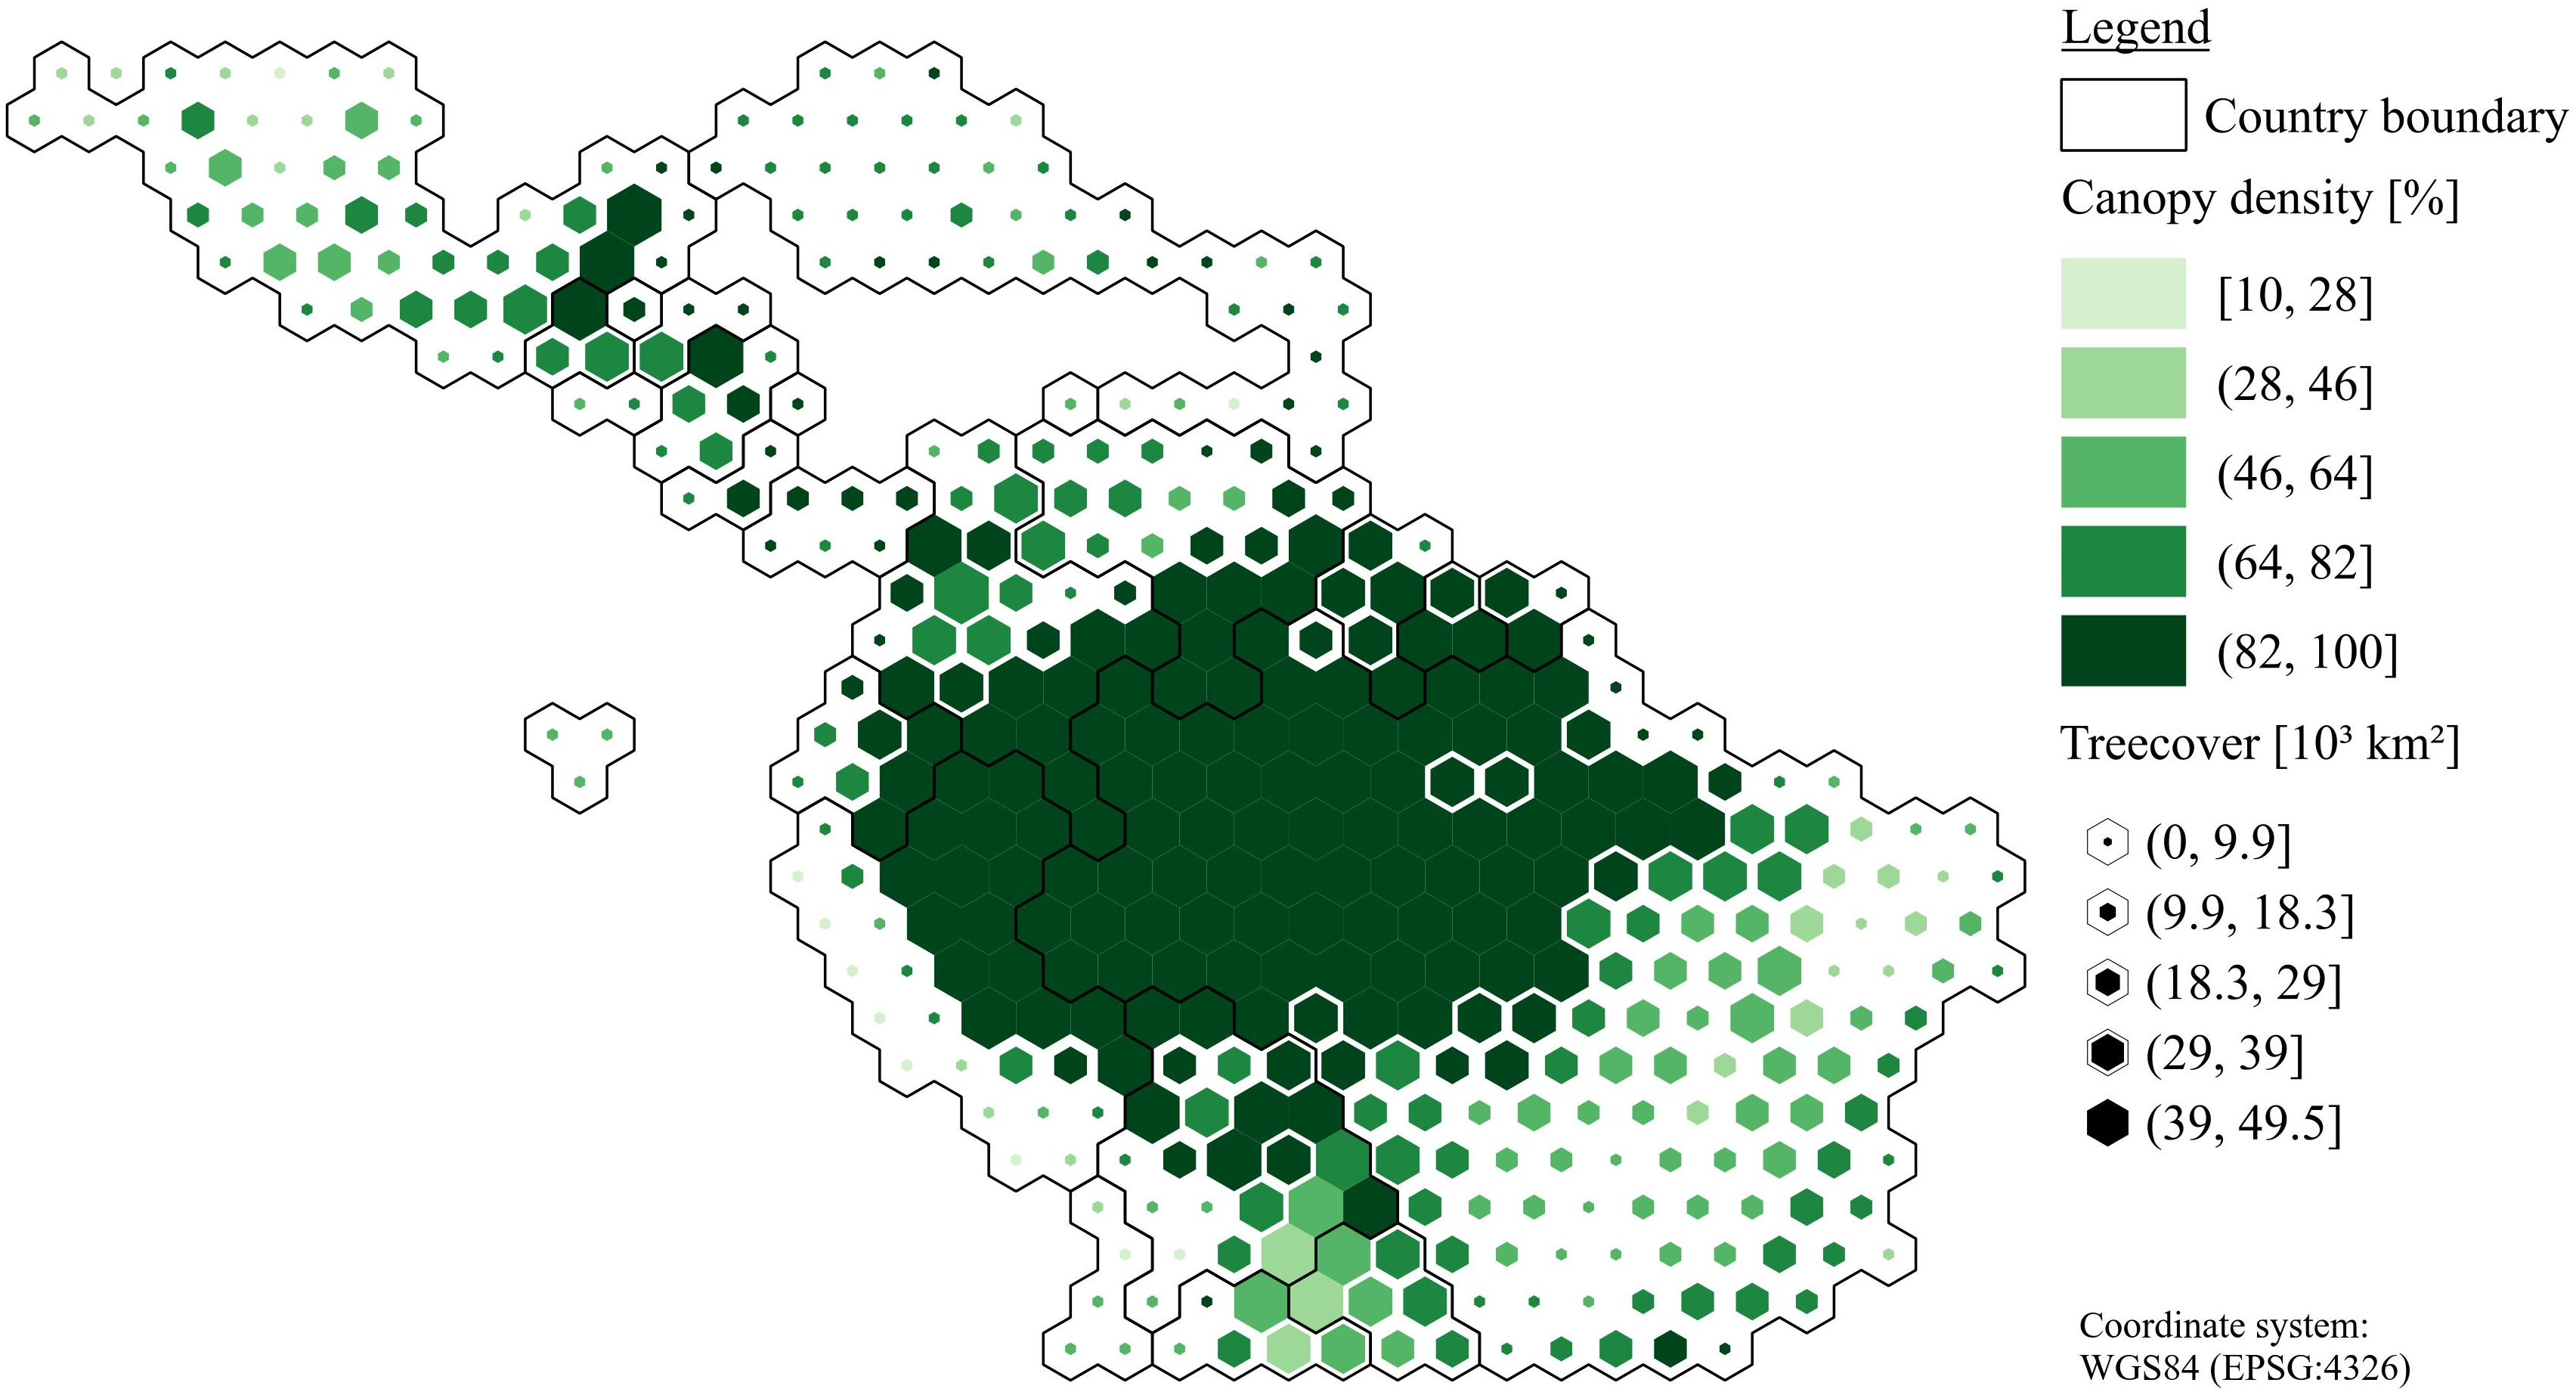
\includegraphics[scale=.91]{img/americas_treecover_frameless}
				\caption[Tree cover and canopy density in Latin America 2000]{\textbf{Tree cover and canopy density in Latin America 2000:} This map shows the tree cover and mean canopy density distribution 2000. An unscaled hexagon covers an area of 0.5 decimal degrees, which translates to an area of approximately 49 thousand km$^2$ at the equator. Tropical rainforest in the center of the map is characterized by a tree cover between approximately 29 and 49 km$^2$ and canopy densities between 82\% and 100\%. The rainforest is surrounded by tropical moist forest with tree cover up to 49 km$^2$ but a lower mean canopy densities between 10\% and 82\% as the rainforest. The tropical dry forest also known as Gran Chaco is located in the lower left of the map distributed over the countries of Bolivia, Paraguay, and Argentina.}
				\label{fig:americas_tree_cover}
			\end{figure}

			The distribution of tree cover loss over Latin America during the 2001-2010 time frame are shown in figure \ref{fig:americas_loss}. During this period an area of approximately 388 thousand km$^2$ is deforested (table \ref{tab:proximate_driver} of appendix \ref{ch:appendix}). We could identify for several countries deforestation hotspots where the deforested area is between approximately 2.7 and 9 thousand km$^2$ as the map suggests. Tropical countries with deforestation hotspots are: Paraguay, Argentina, Bolivia, Brazil, Colombia, Peru, and Guatemala. In Brazil the hotspots of tree cover loss are known as the arc of deforestation. The arc of deforestation covers the Brazilian provinces of Acre, Rond\^{o}nia, Mato Grosso, and Pará, while the deforestation moves into the province of Amazonas \citep{Wood2002}. The tree cover loss within this arc develops along the highway network in this regions \citep{Alves2002,Mueller2016}. Several paved highways like BR-163, BR-219, BR-230 etc. have contributed to the agricultural and infrastructural development and have lead to high deforestation rates. In Brazil an area of approximately 274 thousand km$^2$ was deforested between 2001 and 2010 (table \ref{tab:proximate_driver}). In Paraguay and Argentina the deforestation hotspots are located in the Gran Chaco region, which was once of the least disturbed forests worldwide, but is now exposed to high deforestation rates since 1969 \citep{Caldas2013,Zak2004}. During our study period deforestation accounted for an area of approximately 7097 km$^2$ and 21 thousand km$^2$ in the Argentinian and Paraguayan Chaco, respectively. In Bolivia the deforestation hotspot is located in the department of Santa Cruz. Until the 1960s Bolivia presented relative low deforestation rates, which increased moderately after, and increased sharply during the 1990s and have remained high as the map suggests \citep{Pacheco2002,DavidKaimowitz2002}. During the first decade of 2000s an area of approximately 19 thousand km$^2$ was exposed to tree cover loss. In Guatemala the province of Petén is exposed to deforestation since the 1980s \citep{Beach1998}. Since the 2000s the deforestation rates in Guatemala are among the highest in Latin America and after 2005 the rates increased further \citep{McSweeney2014}. During 2001 and 2010 an area of approximately 6515 km$^2$ is exposed to tree cover loss. \citet{McSweeney2014} highlights that deforestation hotspots often spatially overlap with drug trafficking nodes, especially in the department of Petén where large ranches are owned by narco-traffickers. In Peru deforestation covered the provinces of Huánuco, Loreto, San Martin, and Ucayali, while the cumulative forest loss accounted for an area of approximately 8 thousand km$^2$ in the entire country. An area of approximately 15 thousand km$^2$ is exposed to deforestation in Colombia, while deforestation hotspots are located in Caquetá, Bolívar, and Antioquia.
			\begin{figure}[ht]
				\centering
				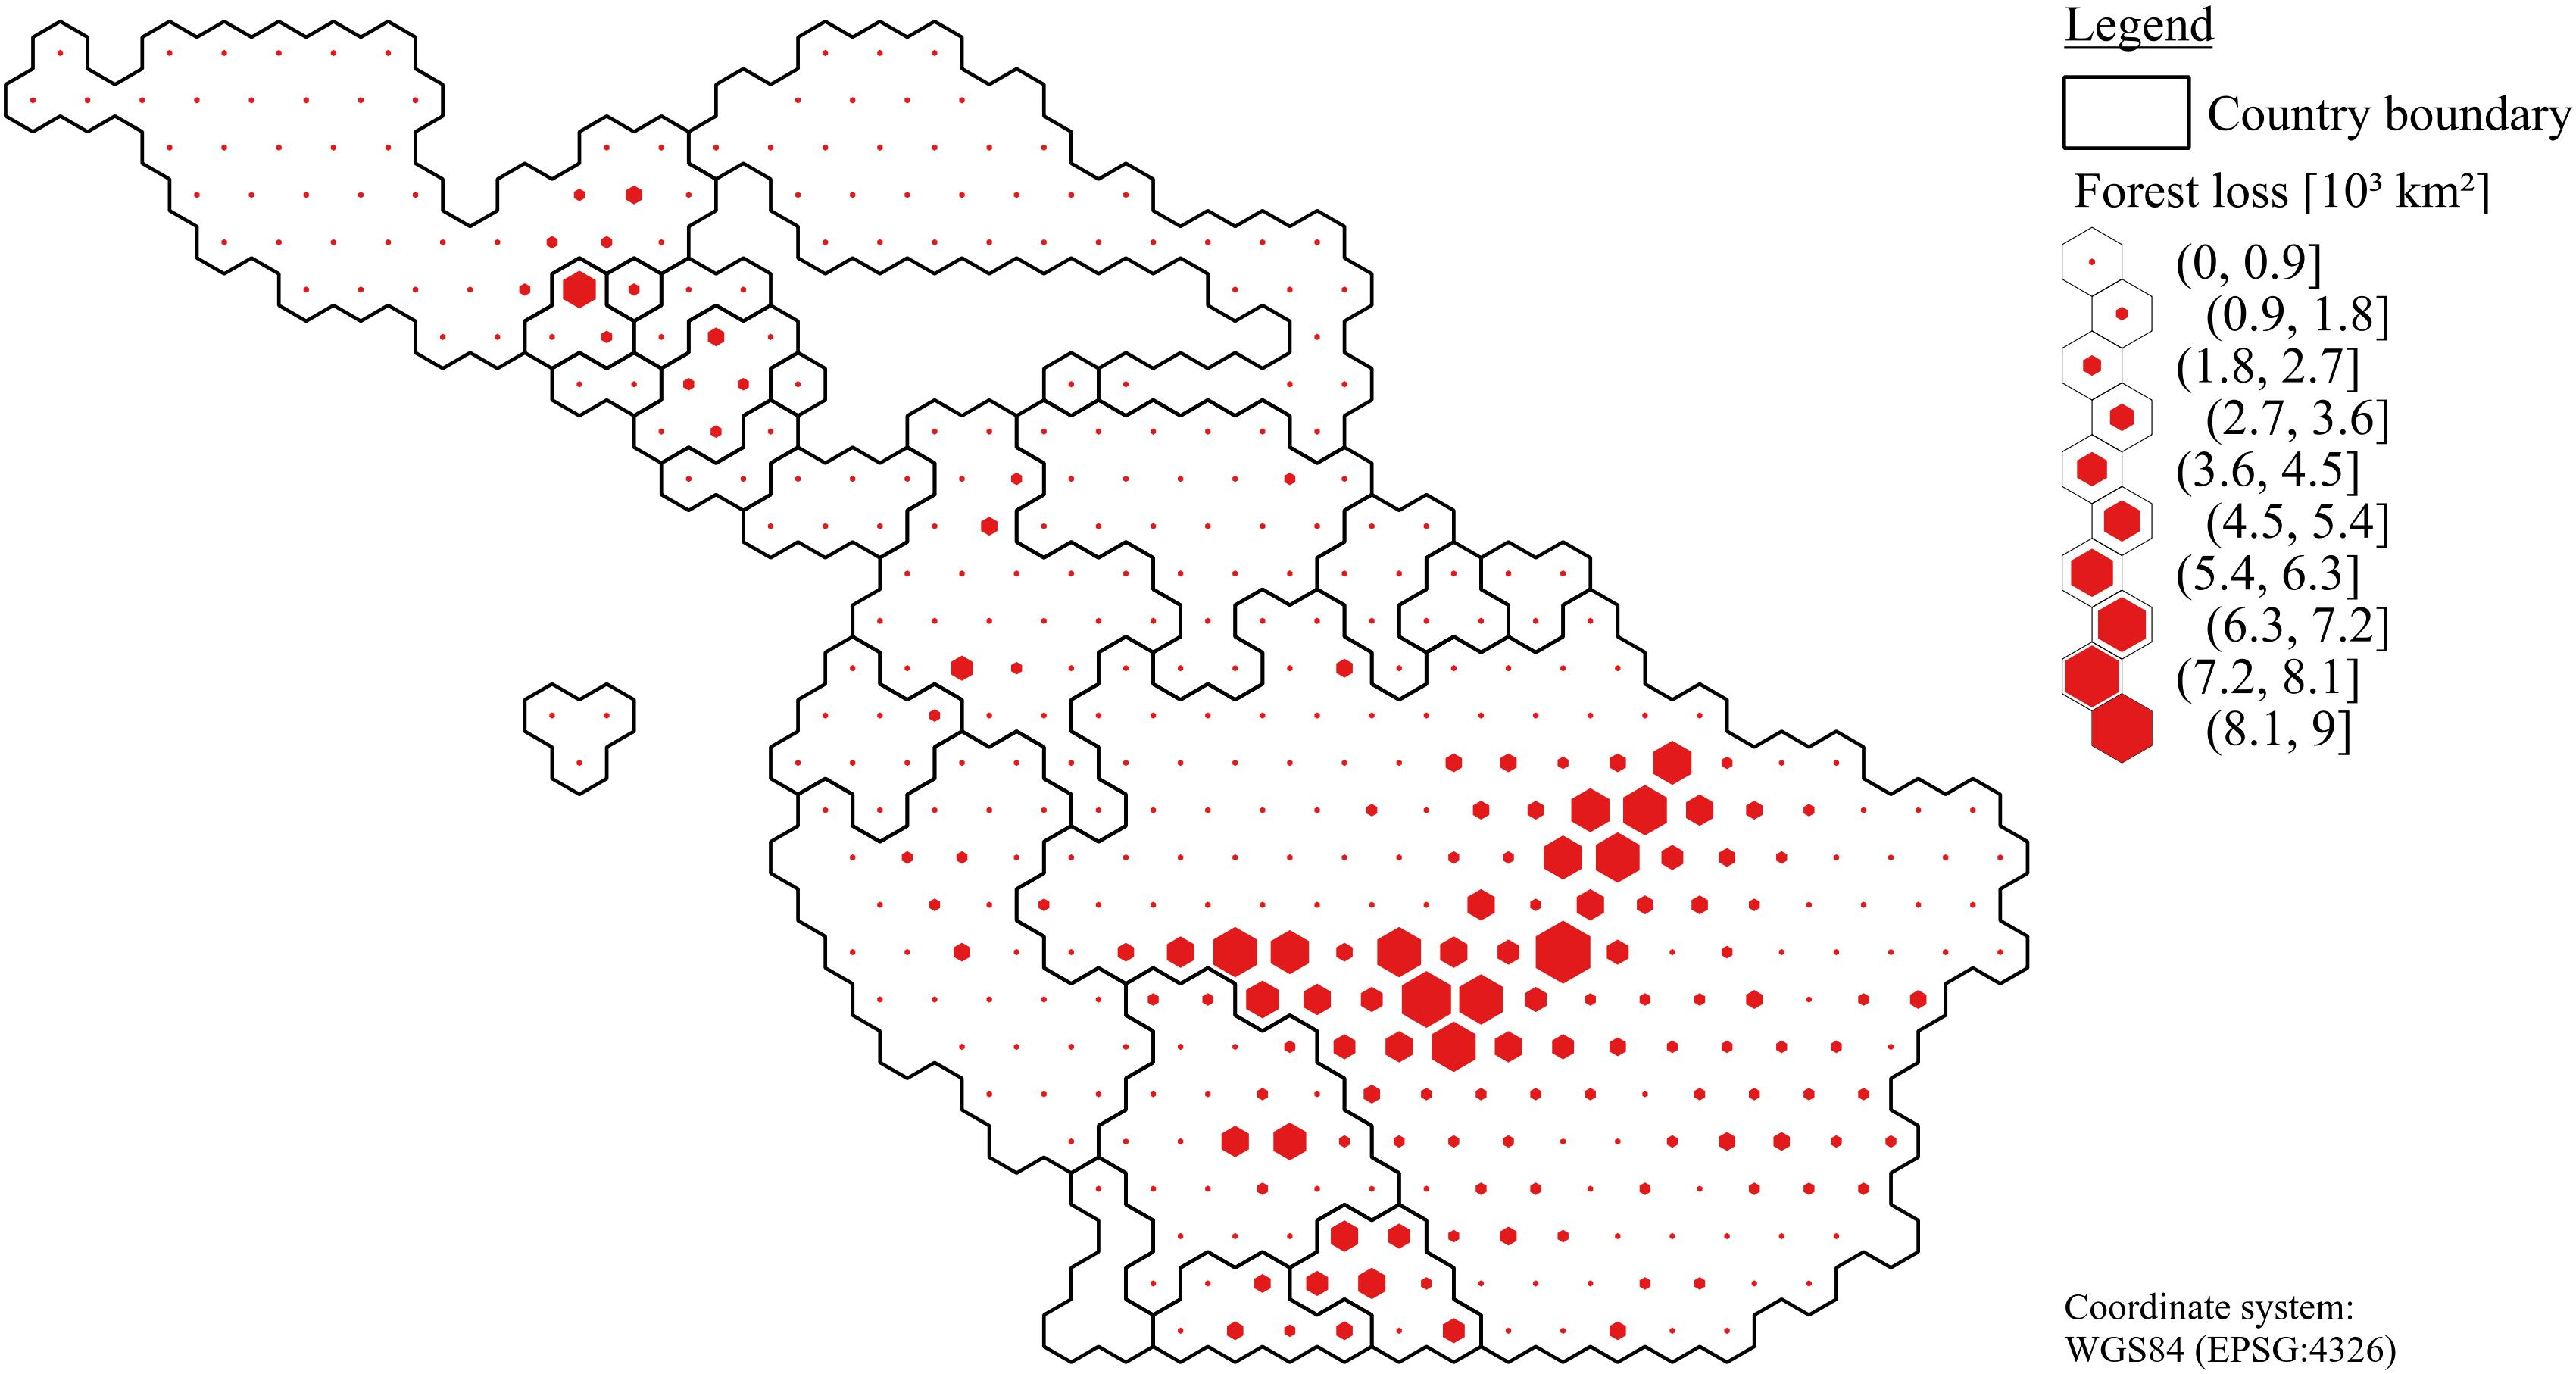
\includegraphics[scale=.91]{img/americas_loss_frameless}
				\caption[Tree cover loss in Latin America between 2001 and 2010]{\textbf{Tree cover loss in Latin America between 2001 and 2010:} This map shows the tree cover loss within our study extent between 2001 and 2010. An unscaled hexagon covers an area of 0.5 decimal degrees, which translates to an area of approximately 49 thousand km$^2$ at the equator. Deforestation hotspots with tree cover loss of about 2.7 thousand km$^2$ per hexagon are located in Paraguay, Argentina, Bolivia, Brazil, Colombia, Peru, and Guatemala.}
				\label{fig:americas_loss}
			\end{figure}

			The tree cover and canopy density distribution for Asia/Australia is presented in figure \ref{fig:asia_tree_cover}. In Asia the tropical rainforest is distributed over several southeast Asian islands like the Indonesian islands of Sumatra, Borneo, Java, Papua. Further rainforest covers the islands of Philippines, Malaysia, and Papua New Guinea. In general the Asian rainforest is characterized by high tree cover coverage per hexagon, which is comparable to Latin America. However, in our map most of the islands are smaller than a single hexagon. Therefore, defined by our method to compute the hexagon scalings the size of the polygons doesn't reflect the tree cover as a share of the landmass and most of them appear smaller. The mean canopy density of tropical rainforest is between 82\% and 100\% and the tree cover is above approximately 9.9 thousand km$^2$. Tropical moist and dry forest are distributed over the continental Asia covering the countries of India, Vietnam, Cambodia, Laos. These forests are characterized by a lower tree cover of about 9.9 thousand km$^2$ and canopy densities ranging between 10\% and 82\%. The lower tree cover indicates that in southeast Asia deforestation occurs since the 1950s \citep{Kummer1994}. 
			\begin{figure}[ht]
				\centering
				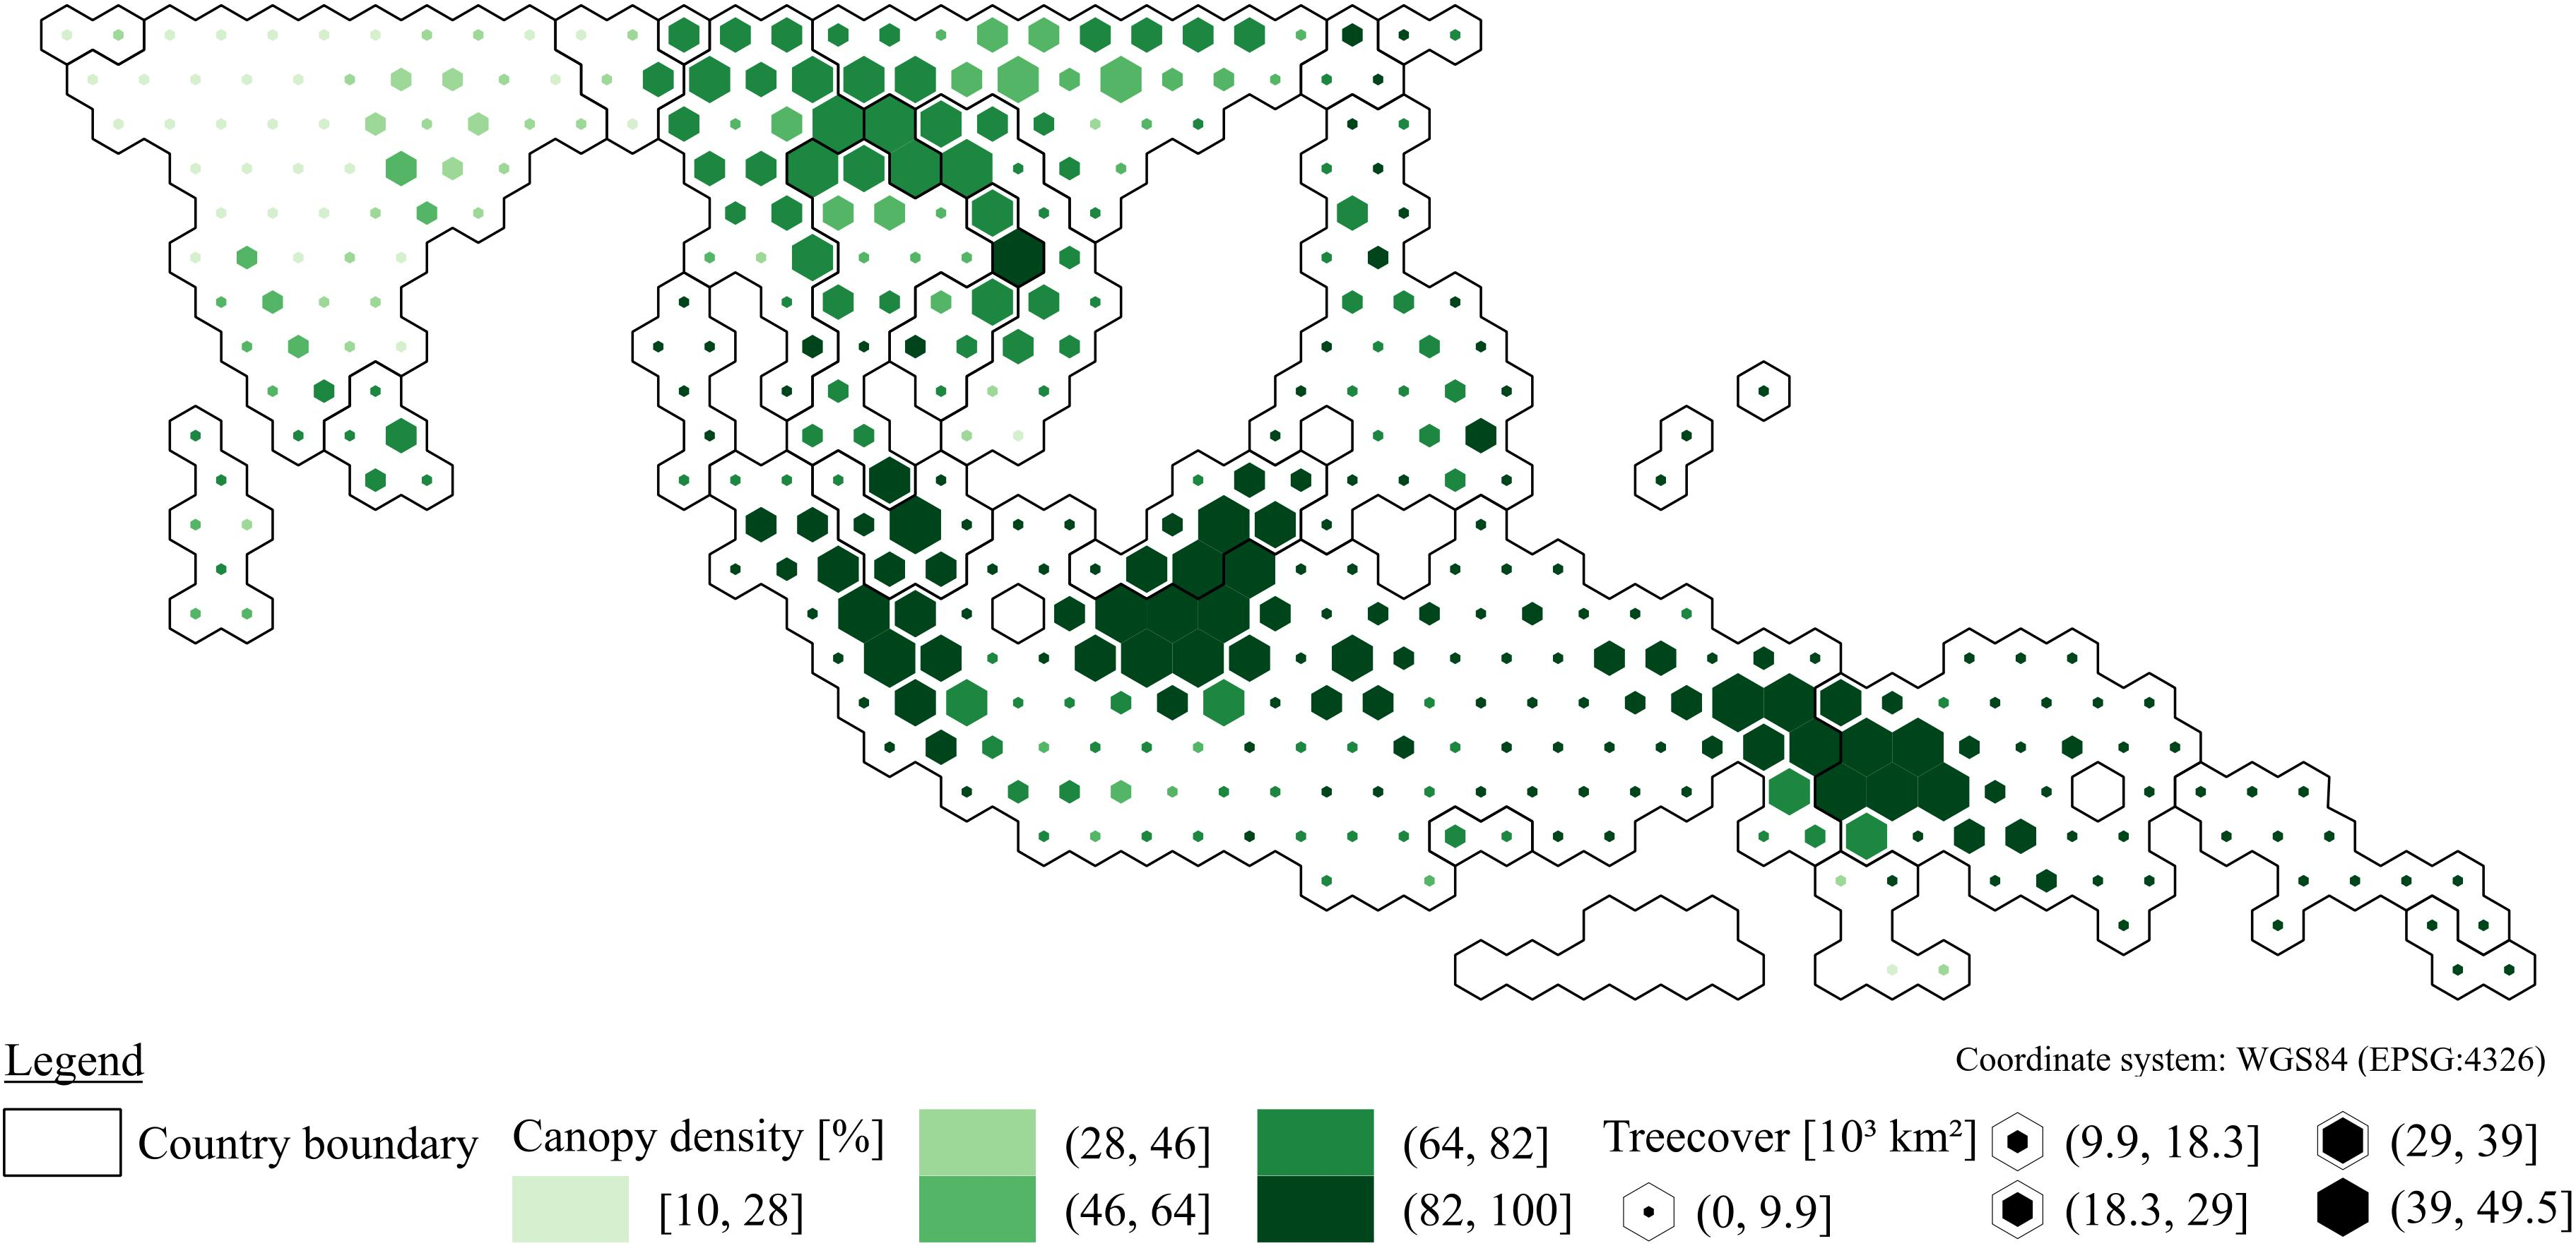
\includegraphics[scale=.91]{img/asia_treecover_frameless}
				\caption[Tree cover and canopy density in Asia/Australia 2000]{\textbf{Tree cover and canopy density in Asia/Australia 2000:} This maps shows the tree cover and mean canopy density distribution within our study extent 2000. An unscaled hexagon covers an area of 0.5 decimal degrees, which translates to an area of approximately 49 thousand km$^2$ at the equator. Tropical rainforest covers largely the Indonesian island system, Malaysia, and Papua New Guinea. This forest type is characterized by a dense canopy between 82\% and 100\%, while the tree cover is above 9.9 thousand km$^2$. Tropical moist and dry forest covers the countries of India, Vietnam, Cambodia, Laos, while the canopy density ranges between 10\% and 82\%.}
				\label{fig:asia_tree_cover}
			\end{figure}

			The figure \ref{fig:asia_loss} shows the distribution of tree cover loss in Asia/Australia for the 2001 till 2010 time period. During this time period a forest area of approximately 196 thousand km$^2$ is exposed to deforestation (table \ref{tab:proximate_driver} in appendix \ref{ch:appendix}). For this region we identified the following countries as deforestation hotspots with tree cover loss areas per hexagon of approximately 1.9 to 9 thousand km$^2$: Indonesia, continental and insular Malaysia, Vietnam, and Laos. Indonesia is known as a country with one of the highest rates of primary forest loss for the time period 2000 till to 2016 \citep{Austin2019}. In the first decade of the 2000s an area of approximately 100 thousand km$^2$ is exposed to deforestation as table \ref{tab:proximate_driver} suggests. The tree cover loss is predominantly distributed over the Indonesian islands of Sumatra and Borneo (the province of Kalimantan) as the map \ref{fig:asia_loss} shows. The Indonesian forests are exposed to changing deforestation causes since the 1950s \citep{Nawir2007}. Malaysia has lost a forest area of approximately 33 thousand km$^2$ by deforestation during the time period 2001 till 2010. The  Malaysian deforestation hotspots are distributed over the Malaysian Borneo (Sarawak/Sabah) and continental Malaysia. Comparable to Indonesia, Malaysia's forests are exposed to deforestation since the 1950s by changing causes like logging followed by agricultural activities \citep{Kummer1994}. From 2001 till 2010 an area of approximately 7 thousand km$^2$ was exposed to deforestation in Vietnam as table \ref{tab:proximate_driver} suggests. We identified the central highland provinces Dak Lak, Dak Nong, Gia Lai, and Lam Dong as deforestation hotspots. \citet{Meyfroidt2013} confirms this in his study on trajectories of deforestation and highlights that the losses in this area could reduce the benefits of national-scale forest recovery. During the early 1990s a transition to reforestation was encouraged and natural forests expanded in Vietnam, while the deforestation increased in the highland regions \citep{Meyfroidt2013,Chazdon2008}. In Laos a forest area of approximately 8 thousand km$^2$ is lost during the time period 2001 till 2010. The map in figure \ref{fig:asia_loss} suggests that northern Laos was predominantly exposed to tree cover loss, which is confirmed by \citet{Hirsch2000}. Laos is known to have experienced a steady loss of forest cover since the early 1960s \citep{Hirsch2000}. The causes for this \ac{LC} transitions have changed over time.
			\begin{figure}[ht]
				\centering
				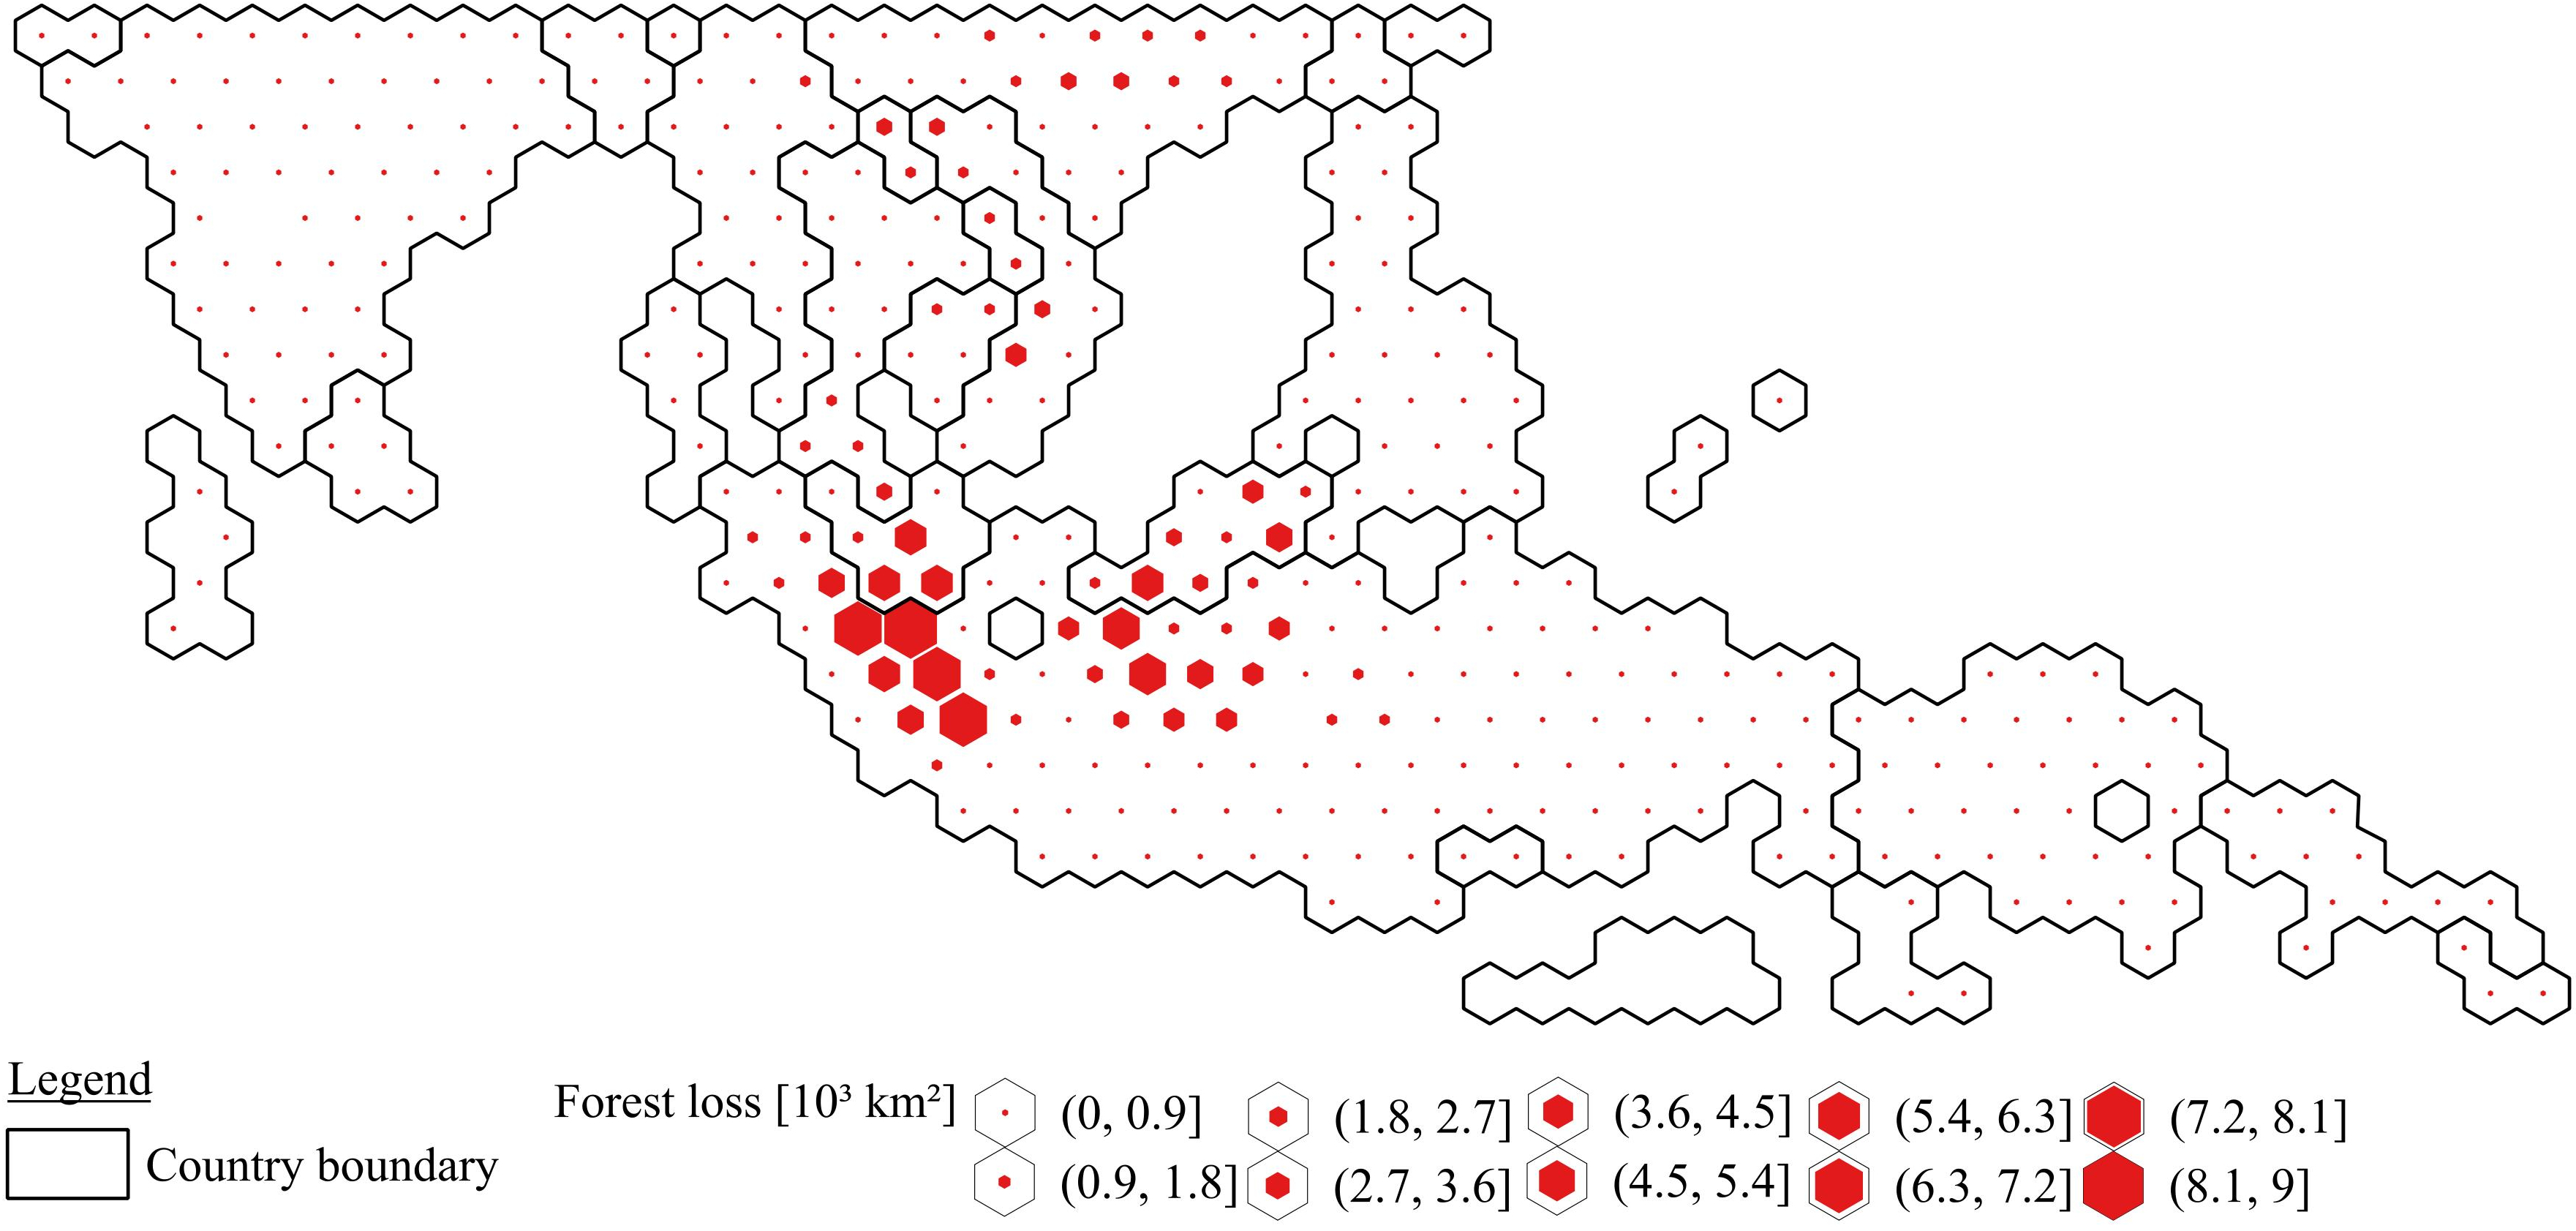
\includegraphics[scale=1.]{img/asia_loss_frameless}
				\caption[Tree cover loss in Asia/Australia between 2001 and 2010]{\textbf{Tree cover loss in Asia/Australia between 2001 and 2010:} This map shows the tree cover loss within our study extent between 2001 and 2010. An unscaled hexagon covers an area of 0.5 decimal degrees, which translates to an area of approximately 49 thousand km$^2$ at the equator. Deforestation hotspots with tree cover loss of about 1.9 thousand km$^2$ per hexagon are located in Indonesia, Malaysia, Vietnam, and Laos.}
				\label{fig:asia_loss}
			\end{figure}

			Figure \ref{fig:africa_tree_cover} shows the tree cover and canopy density distribution over Africa. In Africa the tropical rainforest is distributed over the following central African countries: Democratic Republic of the Congo, Republic of the Congo, Equatorial Guinea, Gabon, Cameroon, and to a lesser degree in Ghana, Ivory Coast, and Liberia. In our map this type of forest is characterized by a dense tree cover between 39 and 49 thousand km$^2$ per hexagon, while the canopy density ranges between 64\% and 100\%. In Africa the canopy density does not separate the moist forest type from the rainforest as good as in Latin America and Asia/Australia. The rainforest is surrounded by tropical moist forest with a dense tree cover coverage per hexagon between 18 and 49 thousand km$^2$, while the mean canopy density ranges between 10\% and 82\%. Countries covered by the moist tropical forest type are the following examples: Angola, Uganda, Central African Republic, Zambia, Madagascar. Tropical dry forest is characterized by a sparse tree cover covering approximately 18 thousand km$^2$ per hexagon and presenting canopy densities between 10\% and 46\%. The countries of Mozambique, Tanzania, and Nigeria are examples for areas which are covered partially by tropical dry forest.
			\begin{figure}[ht]
				\centering
				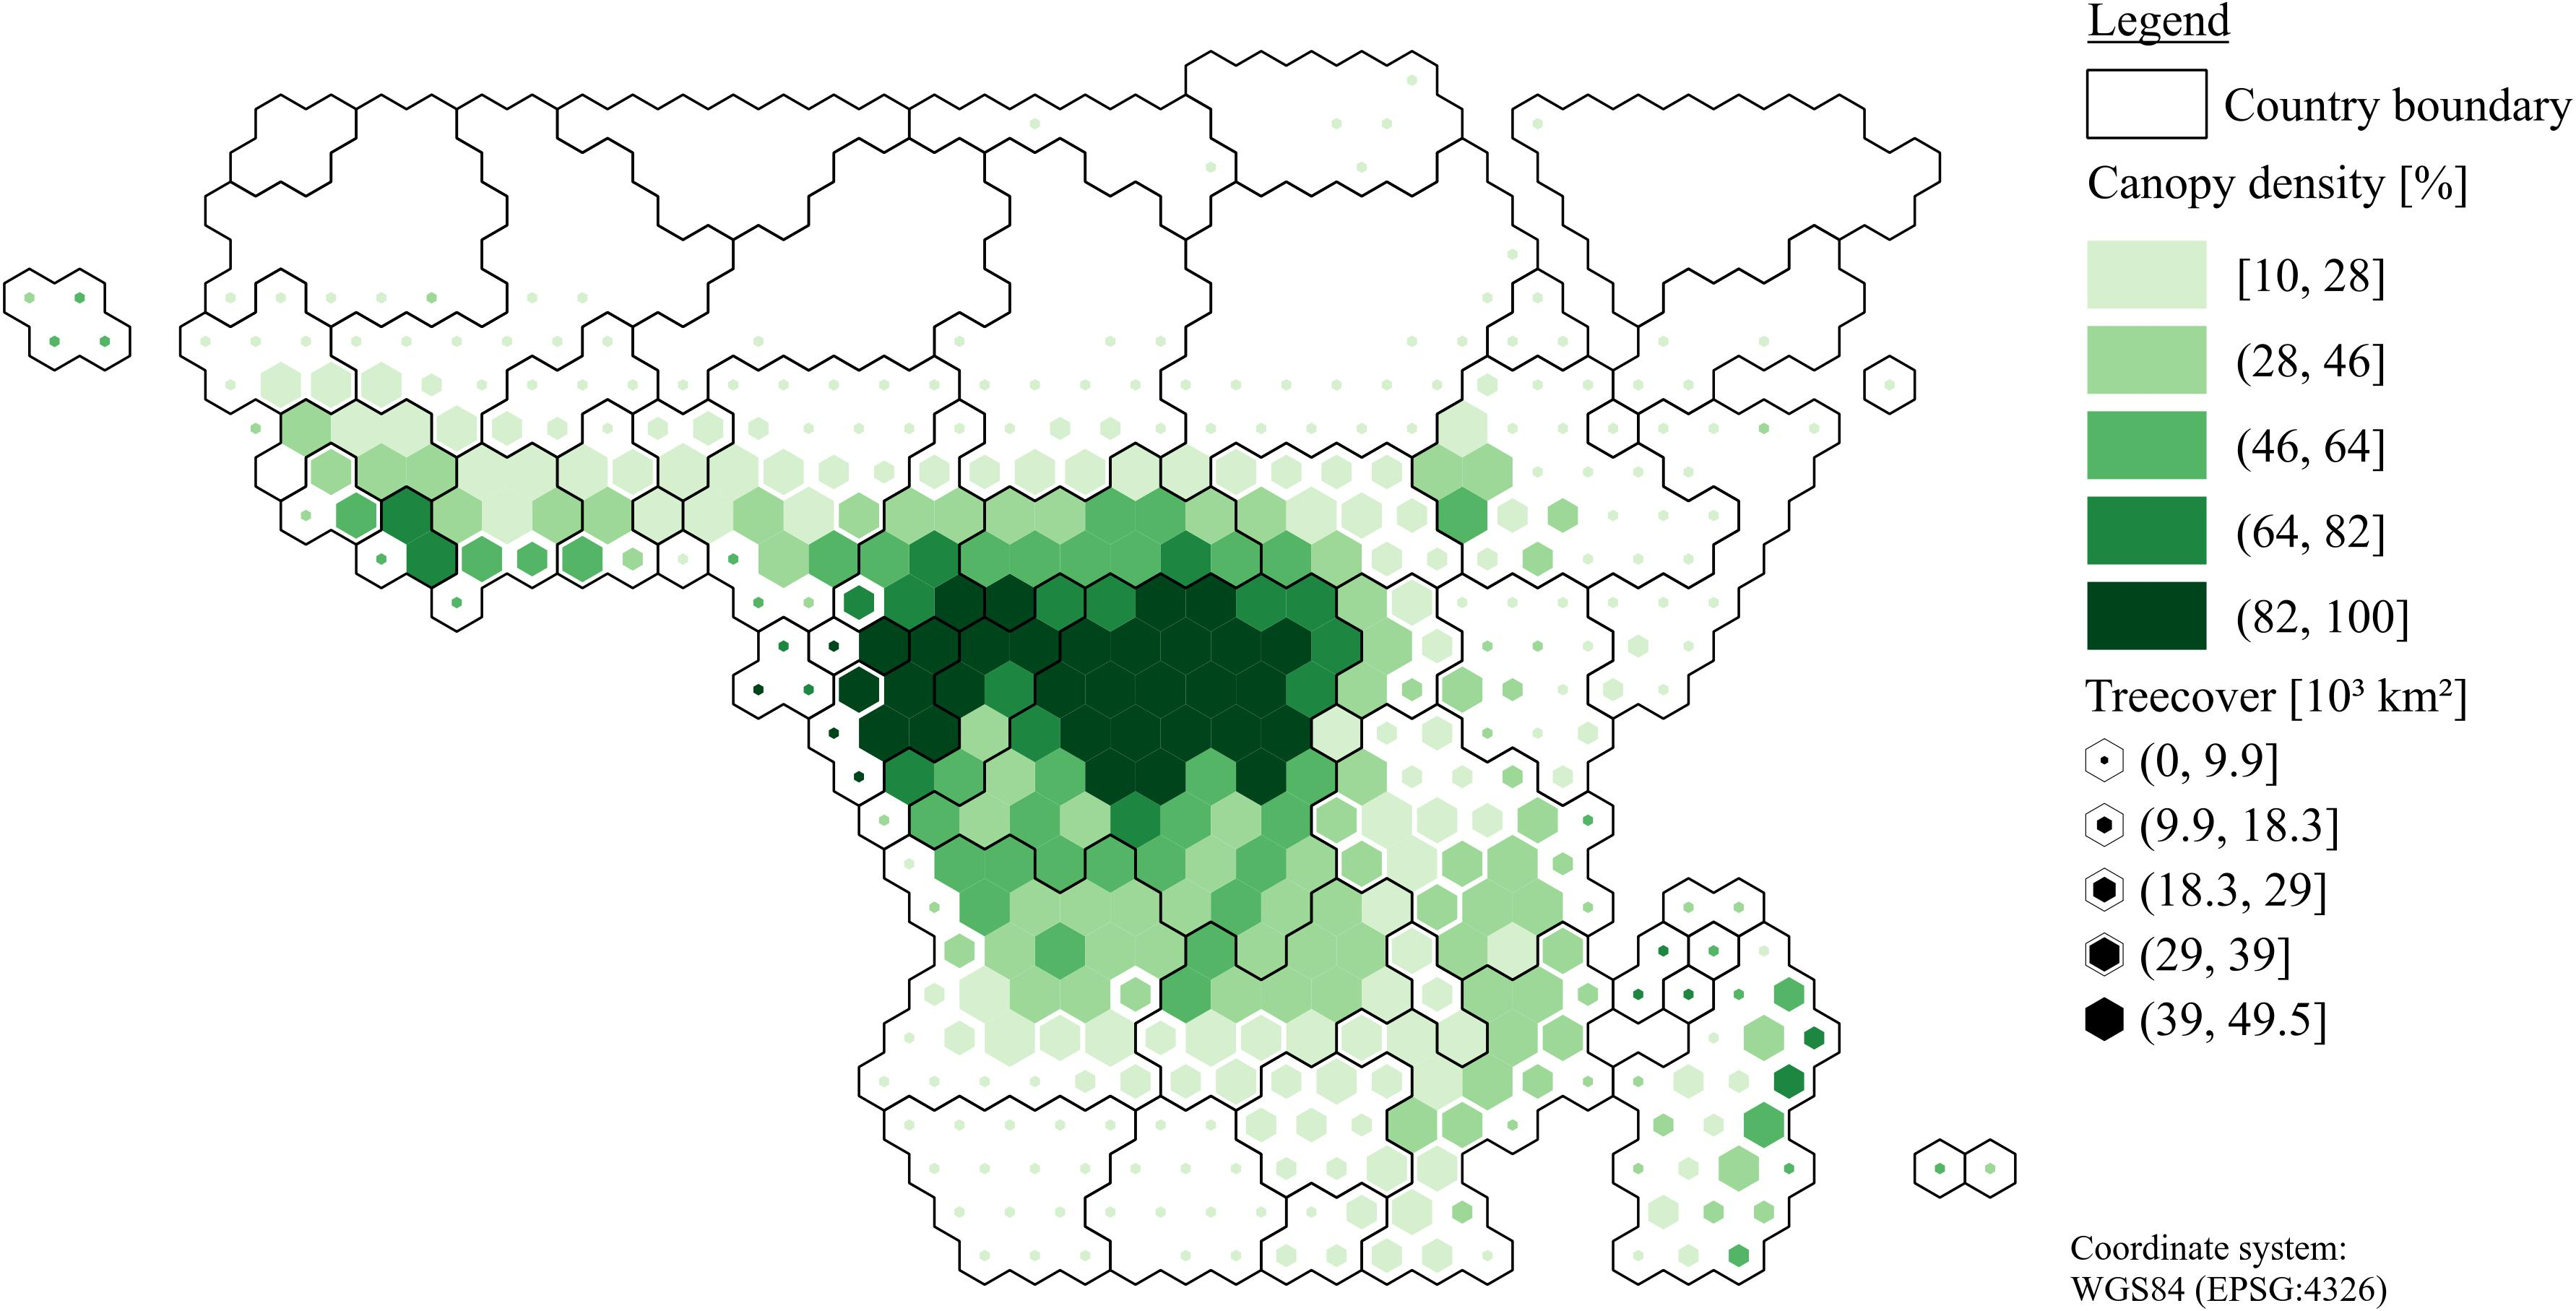
\includegraphics[scale=.91]{img/africa_treecover_frameless}
				\caption[Tree cover and canopy density in Africa 2000]{\textbf{Tree cover and canopy density in Africa 2000:} This maps shows the tree cover and mean canopy density distribution within our study extent 2000. An unscaled hexagon covers an area of 0.5 decimal degrees, which translates to an area of approximately 49 thousand km$^2$ at the equator. Tropical rainforest is characterized by dense tree cover between 39 and 49 thousand km$^2$ and high canopy density above 64\% in the center of Africa. The rainforest is surrounded by tropical moist forest with a dense tree cover as well but a lower mean canopy density between 10\% and 82\%.}
				\label{fig:africa_tree_cover}
			\end{figure}

			For Africa the map in figure \ref{fig:africa_loss} shows the regions which are exposed to tree cover loss for the 2001 till 2010 time period. During the first decade of 2000 an area of approximately 174 thousand km$^2$ was deforested (table \ref{tab:proximate_driver} in appendix \ref{ch:appendix}). With a tree cover loss between 1.1 and 3.7 thousand km$^2$ per hexagon we identified the following countries as deforestation hotspots: Ivory Coast, Democratic Republic of the Congo, Angola, Mozambique, Madagascar, and Tanzania. In Ivory Coast an area of approximately 10 thousand km$^2$ was exposed to deforestation between 2001 and 2010 as table \ref{tab:proximate_driver} shows. The map in figure \ref{fig:africa_loss} shows that the deforestation hotspots are located in the southern and northern parts of the country. Evidences for this are given by \citet{Goetze2006} and \citet{Barima2016}. The comparable lower deforestation rates in the center of the country can be explained by a military conflict started in 2002, which divided the country in a northern and southern zone with a buffer zone in between controlled by United Nation forces and French soldiers \citep{Barima2016}. In Ivory coast continuous loss of tree cover by deforestation started approximately in the 1958s \citep{Chatelain1996}. The deforestation accounts for an area of approximately 45 thousand km$^2$ in the Democratic Republic of the Congo. The Democratic Republic of the Congo is the home of the second largest tropical forest in the world. Compared to other tropical countries it has relatively low deforestation dynamics but recent studies show that deforestation could accelerate in the future \citep{Ickowitz2015}. The deforestation hotspots are located in the eastern Congo and around the medium-sized cities along the Congo river in the lower center of the country. During the first decade of the 2000s an area of about 13 thousand km$^2$ was deforested in Angola. Deforestation hotspots are more oriented to the center of the country covering roughly the provinces Huambo, Bie, and Moxico as the map in figure \ref{fig:africa_loss} suggests. For the time period 1990 till 2009 \citet{Cabral2011} performed a study on forest change in the province of Huambo, where a decrease in dense forest cover is observed, while the cover of sparse forest is increasing \citep{Cabral2011}. Another study by \citet{Schneibel2017} on deforestation dynamics in south-central Angola reveals that the tree cover loss develops along anthropogenic infrastructure and forests are exploited over a long term until a \ac{LC} transitions to other types like cropland occurs. To best of our knowledge no studies on historic deforestation dynamics exist for Angola due to the civil war from 1975 till 2002. In Mozambique an area of approximately 18 thousand km$^2$ was exposed to tree cover loss as table \ref{tab:proximate_driver} suggests. Between 1976 and 1992 during the war, the forests of Mozambique where not largely exposed to deforestation, but since end of the war the deforestation rates are increasing \citep{Sitoe2012}. We identified the following provinces as deforestation hotspots between 2001 and 2010: Zambezia, Nampula, and Cabo Delgado. This is largely confirmed by \citet{Sitoe2012} where it is stated that deforestation is concentrated in the center and north of Mozambique. These hotspots could be related to the higher population densities within this areas. In Madagascar tree cover loss accounts for an area of about 11 thousand km$^2$ during the study period. In Madagascar deforestation hotspots are concentrated at the north-east coast of the island as the map in figure \ref{fig:asia_loss} suggests. Madagascar's central highland forests are exposed to anthropogenic deforestation since the 1600s, reportedly \citep{Harper2007}. By the nineteenth century the deforestation advanced over the entire island forests. In Tanzania an area of approximately 14 thousand km$^2$ was exposed to tree cover loss. Since the 1900s approximately 19.4\% of the forest cover has been lost \citep{Kideghesho2015}. The map in figure \ref{fig:africa_loss} suggests that deforestation hotspots are located in the country center covering the following provinces: Lindi, Singida, Tabora, Dodom, Tanga, Pwani, and the island of Zanzibar.
			\begin{figure}[ht]
				\centering
				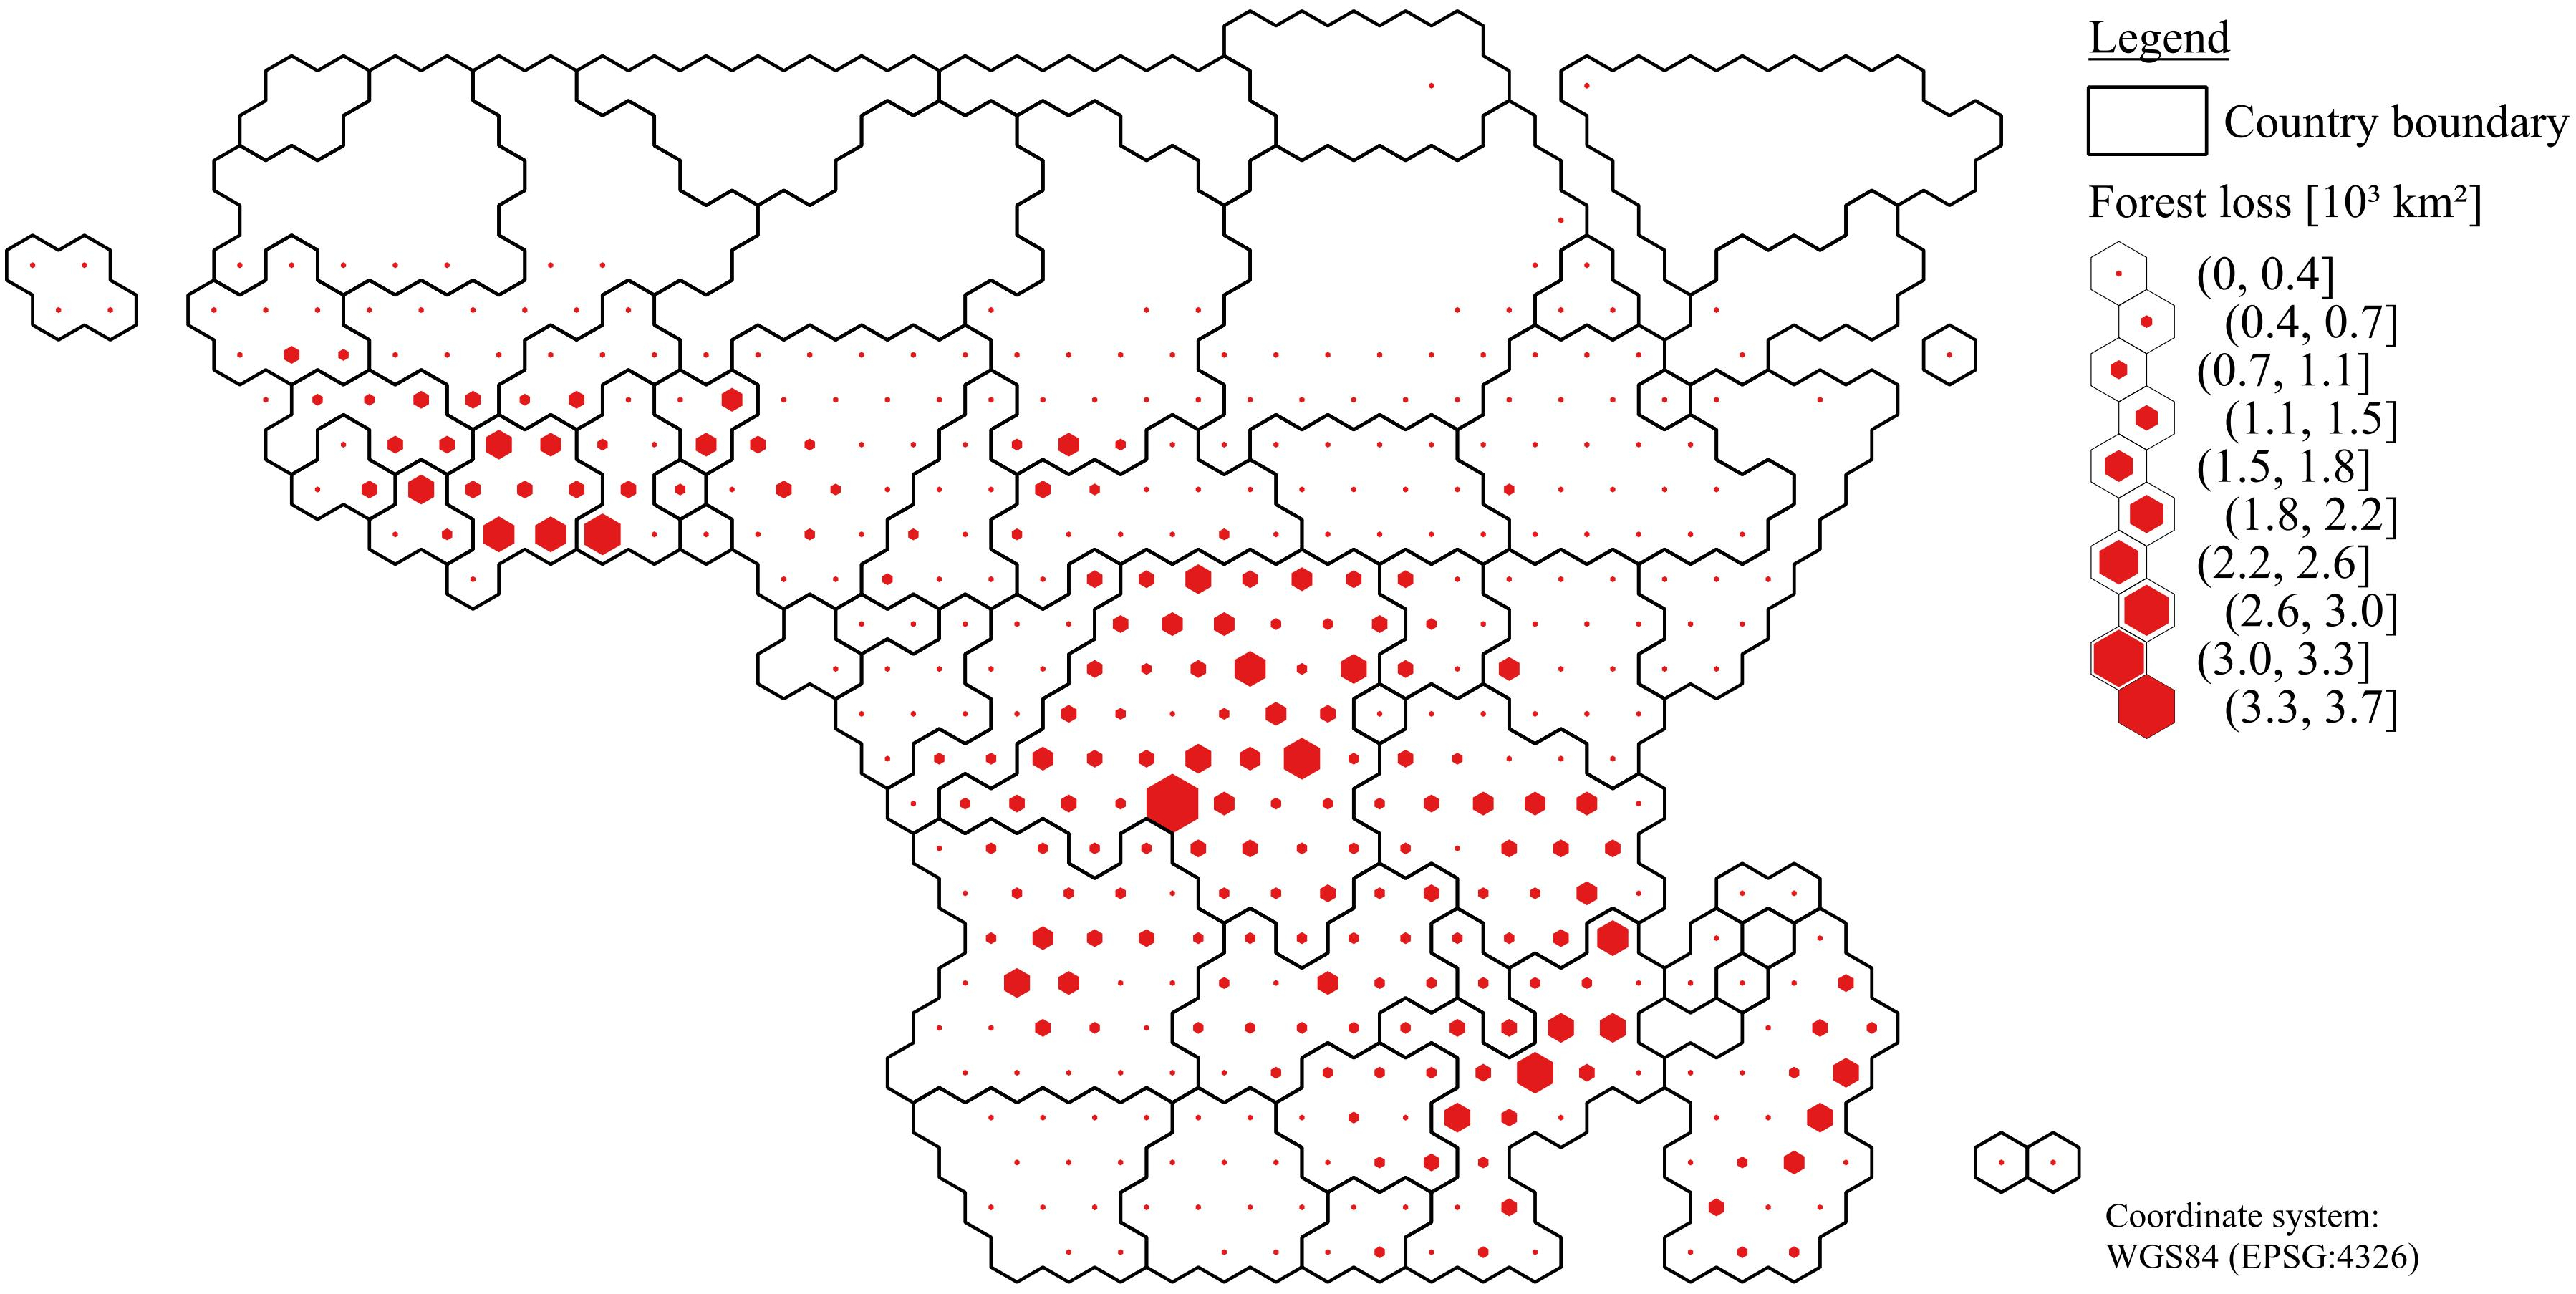
\includegraphics[scale=.85]{img/africa_loss_frameless}
				\caption[Tree cover loss in Africa between 2001 and 2010]{\textbf{Tree cover loss in Africa between 2001 and 2010:} This map shows the tree cover loss within our study extent between 2001 and 2010. An unscaled hexagon covers an area of 0.5 decimal degrees which translates to an area of approximately 49 thousand km$^2$ at the equator. Deforestation hotspots with tree cover loss about 1.1 thousand km$^2$ per hexagon are located in Ivory Coast, Democratic Republic of the Congo, Angola, Mozambique, Madagascar, and Tanzania.}
				\label{fig:africa_loss}
			\end{figure}

		\subsection{Mapping of proximate deforestation drivers}
		\label{subsec:results_proxy_deforestation_drivers}
			In this section we will present the \acp{PDD} of tropical forest cover loss between 2001 and 2010. At first we will discuss the forest changes on the global scale followed by the continental results for Latin America, Asia/Australia, and Africa. During the continental discussion we will refer to countries with deforestation hotspots identified in the previous section. 

			On the global tropical scale the major \acp{PDD} are cropland and pastures, which account for 20.2\% (177,038.5 km$^2$) and 33.1\% (289,445.5 km$^2$) of the tree cover loss (table \ref{tab:proximate_driver} in appendix \ref{ch:appendix}). Regrowth dynamics account for 26.4\% (230,543.7 km$^2$) of the tree cover loss: these dynamics include forestry activities, establishment of plantations, plantation management practices like rotational cycle, and shifting agriculture. The expansion of artificial surfaces accounts for 0.4\% (3,690.1 km$^2$) of the forest loss, while the inundation of forests by rivers and lakes accounts for 1.4\% (12,011.9 km$^2$). For 100 tropical and subtropical countries, \citet{Hosonuma2012} estimates that the expansion of agriculture, mining, infrastructure, and urbanization account for approximately 82\%, 8\%, 8\%, and 2\% of the tree cover loss, respectively. In relation to the \ac{PDD} classification schema of \citet{Geist2001}, the expansion of agriculture relates to cropland, pastures, and plantations in the research of \citet{Hosonuma2012}. Therefore, we receive nearly similar results for agricultural expansion if we would aggregate the classes cultivated, grassland, and regrowth (approximately 79.7\%). The aggregated estimates for the expansion of mining, infrastructure, and urbanization of \citet{Hosonuma2012} are greater than our estimate for the expansion of artificial structures.

			In Latin America the transition of tree cover to cropland and pastures accounted for 21.3\% (95,929.6 km$^2$) and 40.8\% (183,841.4 km$^2$) of the tree cover loss, respectively (table \ref{tab:proximate_driver} in appendix \ref{ch:appendix}). Therefore, approximately 62\% (279,771 km$^2$) of the tree cover is cleared for agricultural purposes in Latin America. Around 12.6\% (56,909.3 km$^2$) of the tree cover loss is followed by tree cover regrowth, while the transition to shrubland accounts for 11.1\% (50,260.2 km$^2$) of the tree cover loss. Minor \acp{PDD} are water, artificial surfaces, and bareland which account for 1.6\% (7,169.9 km$^2$), 0.3\% (1,561.5 km$^2$), and 0.1\% (405.4 km$^2$) of the forest transitions, respectively. \citet{Sy2015} estimate that agriculture accounts for 88.5\% of the tree cover loss, while transitions of forest cover to other \ac{LC} accounts for 11.5\%. \citet{Hosonuma2012} received similar results for the conversion of tree cover to agricultural land, where it accounted for approximately 90\% of the tree cover loss. Both studies estimate that the expansion of artificial surfaces account for approximately 1\% of the forest loss. The large difference could be explained by the definition of the forest transition classes in both studies. In both studies agriculture comprises pastures, cropland, and tree plantations. Further, \citet{Sy2015} use a sample-based approach on 10x10 km \ac{FAO} FRA-2010 RSS data, which could yield overestimates, while \citet{Hosonuma2012} use an empirical approach based on \ac{FAO} data as well. A recent study on \acp{PDD} estimates that commodity-driven deforestation, shifting agriculture, forestry, wildfire, and urbanization account for 56\%, 31\%, 13\%, 1\%, and <1\% of the tree cover loss, respectively \citep{Curtis2018}. Commodity-driven deforestation relates to tree cover loss as long-term permanent transition of forest to a non-forest \ac{LU} like agriculture, which includes cropland, pastures, plantations and so forth. Comparable to the previously mentioned researches on \acp{PDD} the difference between our estimates and \citet{Curtis2018} arise from class definitions. If we would aggregate our \ac{LC} classes to their schema it would yield nearly the same results. In particular the same estimate for tree cover loss by urbanization shows that the similar classes without aggregation yield similar results. 

			In Latin America the \ac{LC} change to cropland is mainly distributed over southern part, while the transition to pastures is concentrated in the central part of the continent as figure \ref{fig:americas_driver} suggests. Cropland expansion mainly took place in the south of Brazil, Paraguay, Argentina, and Bolivia, while forest loss by pasture expansion is concentrated in the center and north of Brazil. The spatial distribution of cropland/pasture dynamics largely corresponds to the findings of \citet{Graesser2015}. Large quantities of tree cover regrowth can be observed in the south-east and center of Latin America, namely the southeast coast of Brazil, and within the tropical rainforest covering Brazil, Peru, and Colombia. In south-east Brazil the findings of \citet{Curtis2018} suggests that the regrowth dynamics are driven by forestry actions, while the coastline is exposed to shifting agriculture. Cropland and pasture expansion account for 19.1\% and 49.7\% of the tree cover loss, while regrowth dynamics and artificial surfaces account for 11.8\% and 0.3\% of the tree cover loss in Brazil, respectively. 

			Figure \ref{fig:americas_driver} shows that deforestation by cropland expansion is mainly concentrated in the southern part of Brazil in the provinces Mato Grosso, Goi\'{a}s, and Mato Grosso do Sul, which is largely confirmed by \citet{Zalles2018} and \citet{Graesser2015}. Additionally, in the northern part of Mato Grosso and the southern part of Mato Grosso do Sul deforestation by grassland expansion can be observed \citep{Graesser2015,Sy2015}. The tree cover loss in the arc of deforestation can be attributed to pasture expansion, which is again confirmed by \citet{Sy2015} and \citet{Graesser2015}. For the Chaco region of Paraguay the main \ac{PDD} is the expansion of cropland, which accounts for 48.9\% of the tree cover loss. The findings of \citet{Graesser2015} and \citet{Caldas2013} suggest that the main \ac{PDD} in this region is the expansion of pastures, while findings by \citet{Graesser2018} suggests that pastures are largely replaced by cropland \ac{LU} between 1990 and 2015. Therefore, the initial cause for tree cover loss could be the expansion of pastures, but the \ac{LU} has already changed to cropland at our image date of 2010. In the Argentinian part of the Chaco cultivated and grassland account for 65.8\% and 5.3\% of the tree cover loss. This could also be observed by \citet{Sy2015}. In Bolivia cropland and pasture expansion account for 37.2\% and 22.4\% of the forest loss, respectively, while transitions of forest cover to artificial surfaces account for 0.4\% of the tree cover loss. The main \ac{PDD} for the deforestation hotspot in the province Santa Cruz is the expansion of cropland as figure \ref{fig:americas_driver} suggests. Further, in north Bolivia and at the Brazilian border the deforestation is driven by pasture expansion. Both patterns are largely confirmed by \citet{Graesser2015} and \citet{Sy2015}. In Guatemala cropland, pasture, and artificial expansion account for 23.9\%, 38.6\%, 0.5\% of the forest loss, respectively. The main \acp{PDD} for the deforestation hotspot in the province of Peten are pasture expansion followed by cropland expansion as the map \ref{fig:americas_driver} suggests. Pasture expansion is the main force for deforestation in Southern Guatemala. Regrowth dynamics in Guatemala, which account for 12\% of the forest loss, could be attributed to the establishment of oil palm plantations and shifting agriculture \citep{Furumo2017,Curtis2018}. In Peru cropland, pasture, and artificial expansion account for 6.6\%, 23\%, and 0.2\% of the forest loss, while regrowth dynamics account for 28.2\% of the forest loss, respectively. For the deforestation hotspots located in the provinces of Huánuco, San Martin, and Ucayali the major \acp{PDD} are the expansion of pastures and regrowth dynamics. \citet{Sy2015} findings suggests that the expansion of cropland is the main deforestation driver in this central region of Peru. Regrowth dynamics in this region could be related to deforestation for oil palm plantations as the findings of \citet{Vijay2018} and \citet{Furumo2017} suggest. \citet{Vijay2018} estimate that an area of approximately 845 km$^2$ is cleared for oil palm plantations between 2007 and 2013, while \citet{Furumo2017} states that approximately a forest area of 156 km$^2$ was cleared for palm oil plantations between 2001 and 2014. Cultivated land, grassland, and regrowth dynamics account for 6.2\%, 33.4\%, and 24.7\% of the tree cover loss in Colombia, respectively. For the Colombian deforestation hotspot located in the province of Caquetá the expansion of pastures is the main \ac{PDD}, which is confirmed by \citet{Graesser2015}. This is also the case for the deforestation hotspots located in the provinces of Bolívar and Antioquia.
			\begin{figure}[ht]
				\centering
				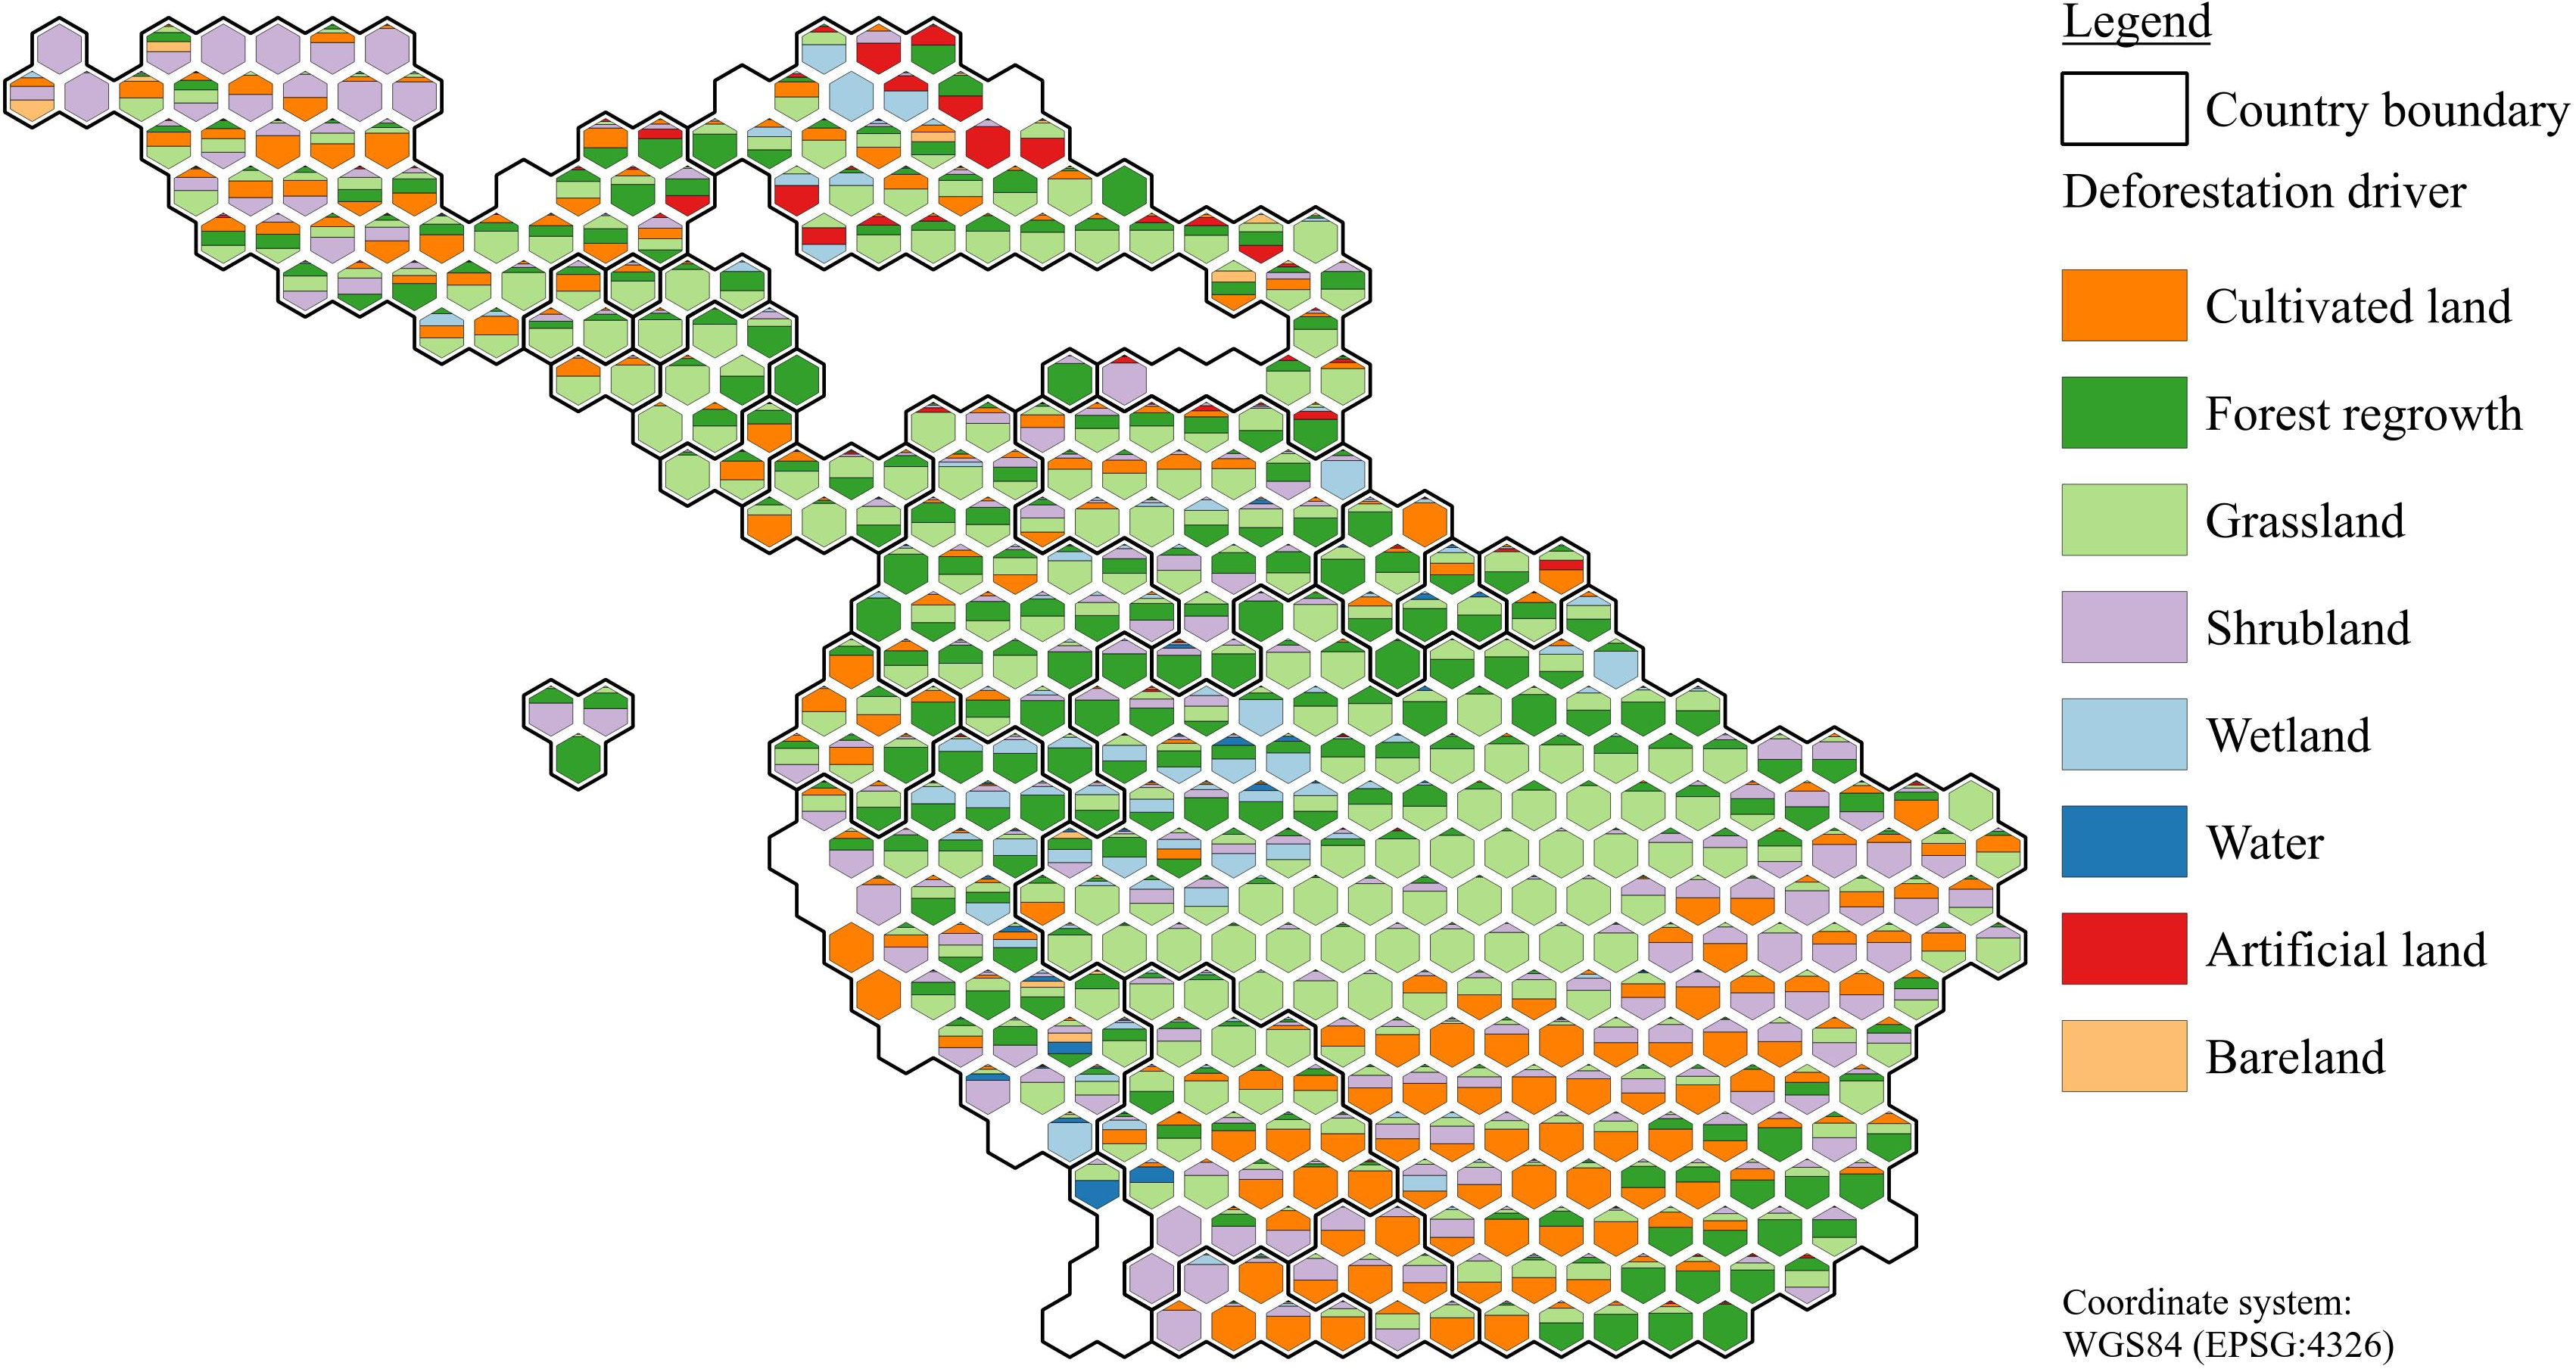
\includegraphics[scale=1]{img/americas_driver_frameless}
				\caption[Map of proximate deforestation drivers in Latin America]{\textbf{Map of proximate deforestation drivers in Latin America:} The map shows the distribution of proximate deforestation drivers in Latin America. The different sized and colored quantities within each hexagons interior shows the relative tree cover loss by a proximate deforestation driver. Scaling of a the hexagons is only intended for improving visual appeal of \acp{PDD}.}
				\label{fig:americas_driver}
			\end{figure}

			For Asia/Australia the table \ref{tab:proximate_driver} in the appendix \ref{ch:appendix} shows that the expansion of cultivated and grassland account for 16\% (36,819.3 km$^2$) and 7.1\% (16,302.6 km$^2$) of the tree cover loss, respectively. Therefore, the transition of \ac{LC} to agriculture usage accounts for 23.1\% (53,121.9 km$^2$) of the tree cover losses. The transition of tree cover to artificial surfaces and the forest loss by inundation of lakes and rivers accounts for 1.1\% (2,431.9 km$^2$) and 0.4\% (890 km$^2$), respectively. In Asia/Australia the largest \ac{PDD} is the regrowth which accounts for 61.2\% (140,653.4 km$^2$) of the cumulative tree cover loss. Forest transitions to shrubland account for 6.7 \% (2,146.2 km$^2$). \citet{Hosonuma2012} estimates that \ac{LC} transitions by agriculture account for approximately 70\% of the forest loss, while \citet{Curtis2018} estimates that commodity-driven deforestation, shifting agriculture, forestry, wildfire, and urbanization account for 13\%, 78\%, 9\%, 13\%, <1\%, and <1\% of the tree cover loss in Southeast Asia, respectively. As mentioned in the previous paragraph the differences in \acp{PDD} estimates relate mainly to the applied methodology and the aggregation of \ac{LC} classes. 

			The figure \ref{fig:asia_driver} shows an overview of the \acp{PDD} distribution in Asia/Australia and indicates that regrowth dynamics are largely concentrated at the east of Asia/Australia, namely in the following countries: Indonesia, Malaysia, Philippines, and Papua New Guinea. Conversion of tree cover to cropland can be observed in Vietnam, Cambodia, the north of Thailand, and India in its entire extent. \citet{Curtis2018} predicts that in Indonesia and Malaysia tree cover loss is largely driven by commodity-driven deforestation, while in Vietnam and Cambodia the forest loss is driven by commodity-driven deforestation and forestry. 

			In Indonesia cropland and pasture expansion accounts for 15.4\% and 4.6\% of the forest cover loss, respectively, while regrowth dynamics account for the largest share of forest loss with 68.6\%. For the deforestation hotspots concentrated on the Indonesian islands of Sumatra and Borneo (the province of Kalimantan) the major \ac{PDD} are regrowth dynamics. This \ac{LC} transitions could be attributed to forest clearings for oil palm plantations and the rotational cycle of matured plantations which are commonly cleared after 18 years \citep{Corley2016}. \citet{Corley2016} estimates that by 2010 an area of approximately 81 thousand km$^2$ is covered by palm oil plantations. \citet{Austin2019} estimates that forestry activities and oil palm plantations account for 67\% of the tree cover loss, while agricultural expansion account for 35\% of the forest transitions in Indonesia between 2001 and 2015. For the islands of Sumatra and Borneo \citet{Austin2019} predicts that more than a half of deforestation could be attributed to forestry and oil palm plantations. In Malaysia regrowth dynamics account for the largest share of forest loss with 79.4\% of the tree cover loss. The cropland and grassland expansion accounts for 7.5\% and 2.6\% of the tree cover loss, respectively. The deforestation hotspots are largely dominated by regrowth dynamics, which again are likely attributed to palm oil plantations and the related management practices like establishment of new sites and clearing of matured plantations. The establishment of new sites is unlikely because the Malaysian industry has difficulties in finding appropriate sites for further expansion \citep{Corley2016}. \citet{Corley2016} reports that by 2015 an area of approximately 50 thousand km$^2$ is covered by palm oil plantations in Malaysia. In Vietnam the \acp{PDD} cropland and pastures account for 32.8\% and 18.3\% of the tree cover loss, respectively. Further, regrowth dynamics account for 30.8\% of the tree cover loss. The deforestation hotspots concentrated in the highlands are dominated by transitions to cropland, while the remaining part of the country is dominated by regrowth dynamics. The regrowth could be related to an increased reforestation effort \citep{Chazdon2008}. \citet{Curtis2018} predicts for the highland region that tree cover loss mainly can be attributed to commodity-driven deforestation. Cropland and pasture expansion account for 14.8\% and 16.4\% of the tree cover loss, respectively, while regrowth dynamics account for 57\% of the forest loss in Laos. The north and south of the country are dominated by regrowth dynamics, while the expansion of cropland is the second largest cause of deforestation. \citet{Curtis2018} data shows that the north is dominated by forestry activities and the south by commodity-driven deforestation.
			\begin{figure}[ht]
				\centering
				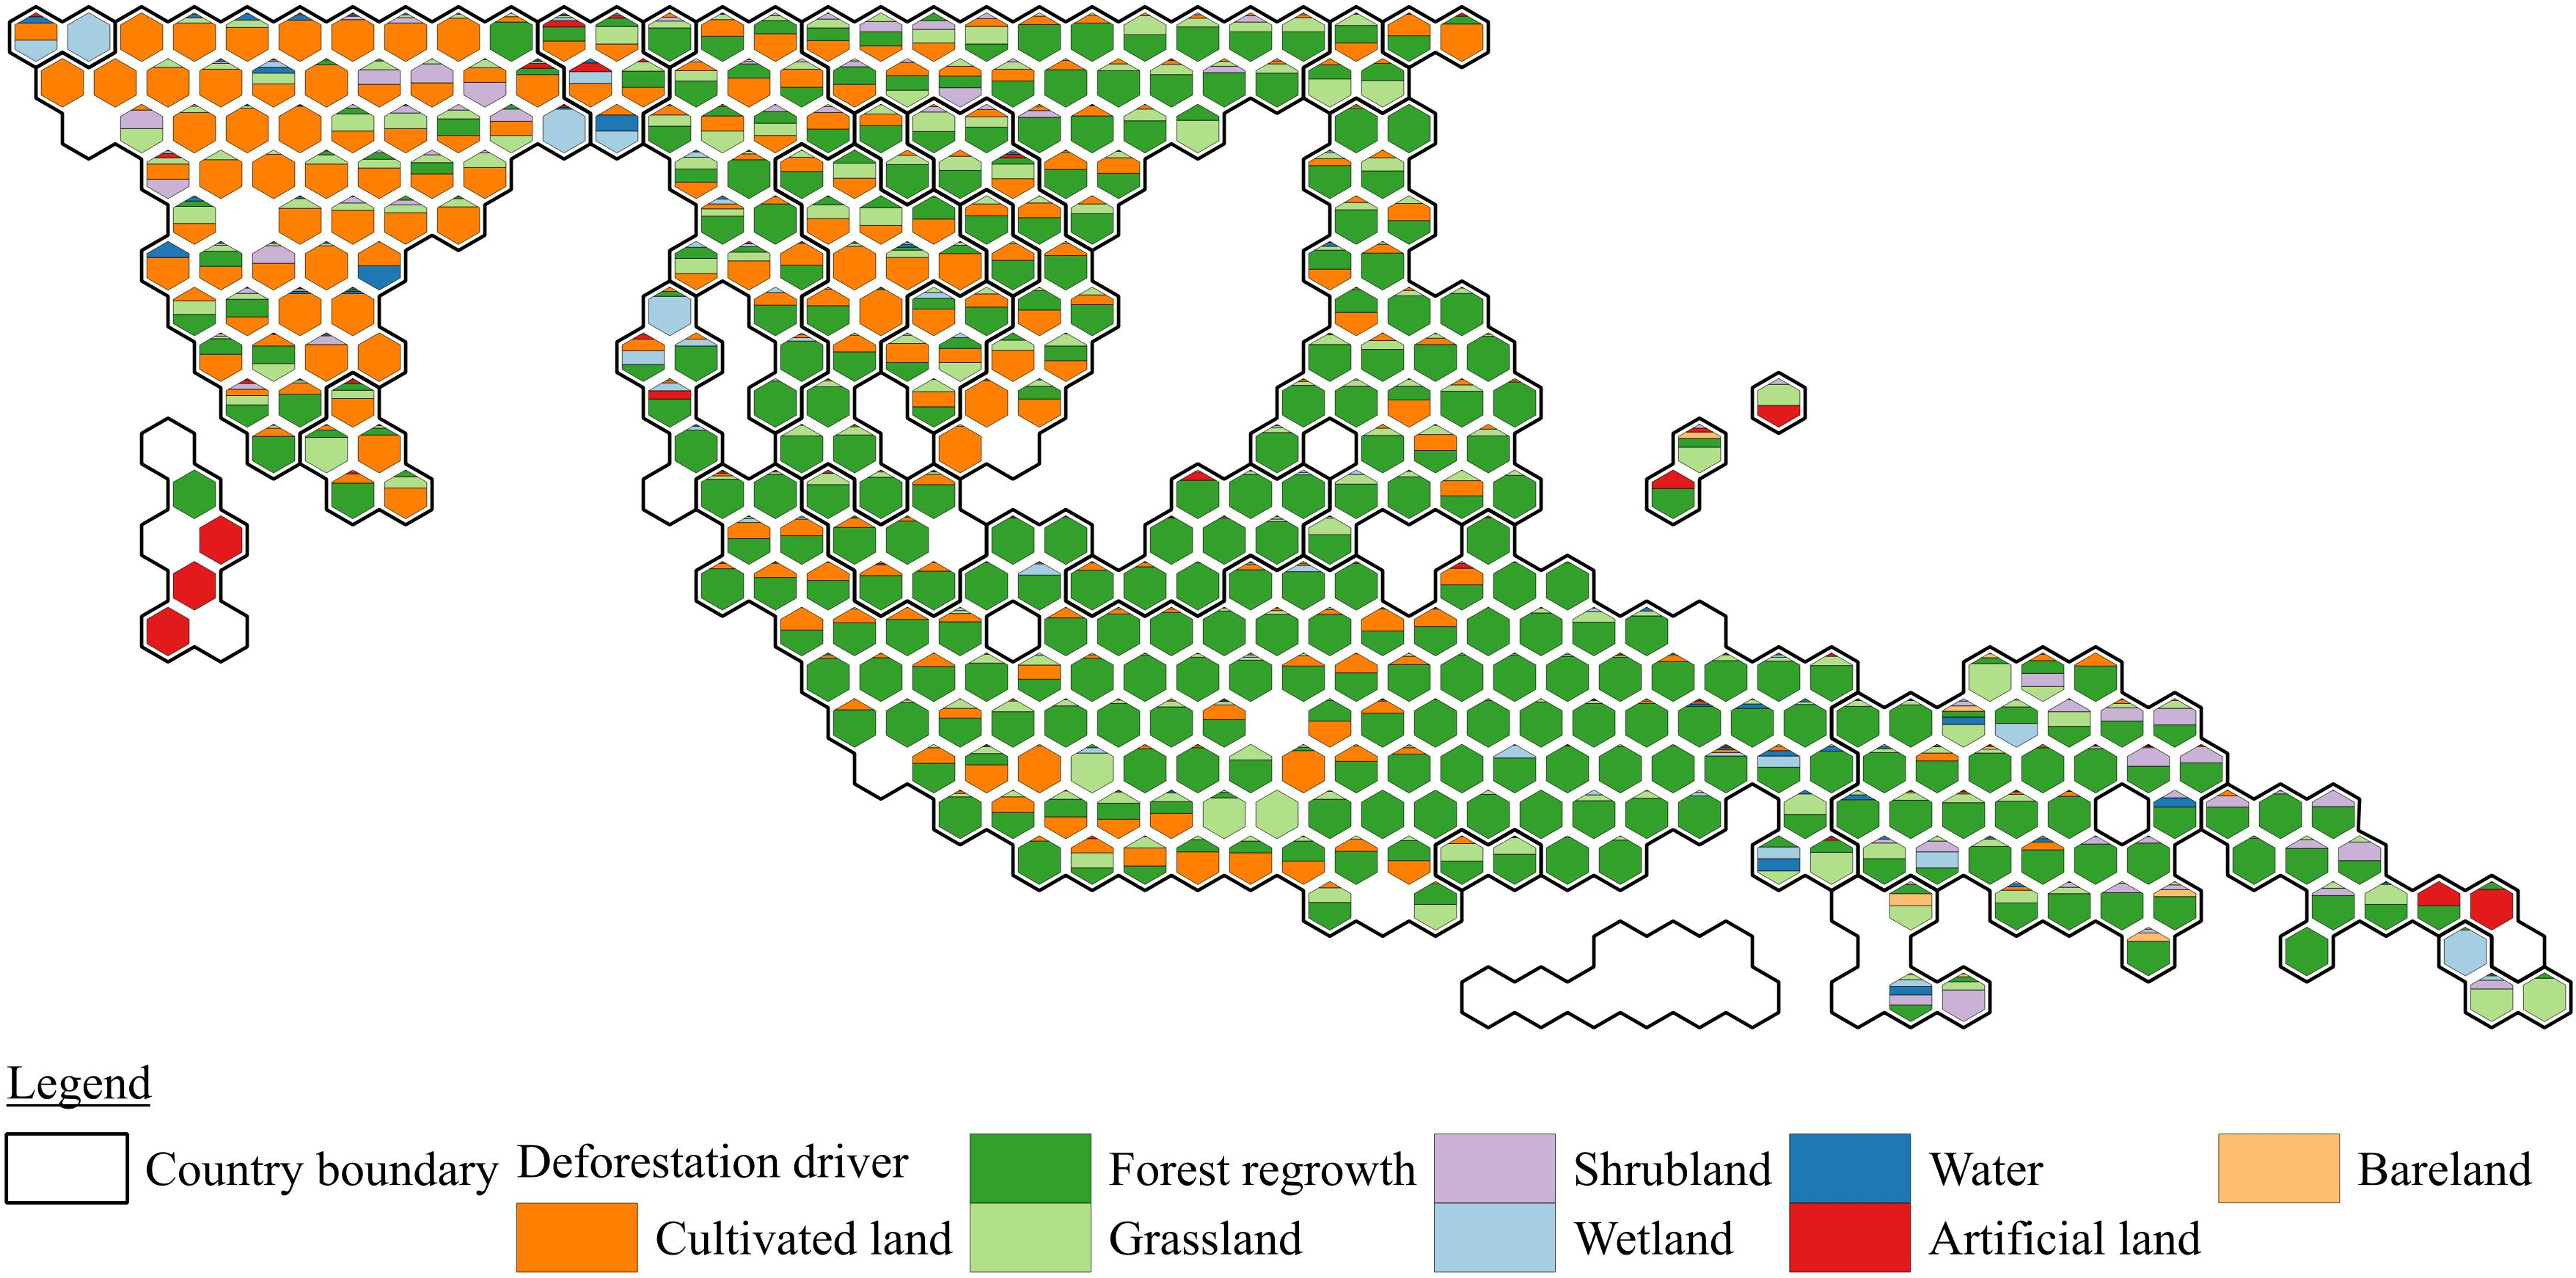
\includegraphics[scale=1]{img/asia_driver_frameless}
				\caption[Map of proximate deforestation drivers in Asia/Australia]{\textbf{Map of proximate deforestation drivers in Asia/Australia:} The map shows the distribution of proximate deforestation drivers in Asia/Australia. The different sized and colored quantities within each hexagons interior shows the relative tree cover loss by a proximate deforestation driver. Scaling of a the hexagons is only intended for improving visual appeal of \acp{PDD}.}
				\label{fig:asia_driver}
			\end{figure}

			In Africa the table \ref{tab:proximate_driver} in the appendix \ref{ch:appendix} suggests that cropland and grassland expansion accounts for 22.8\% (44,289.5 km$^2$) and 46\% (89,301.4 km$^2$) of the tree cover loss, respectively. Therefore, transitions to agricultural land is the major \ac{PDD} in Africa and accounts for 68.8\% (133,590.9 km$^2$) of the tree cover loss. Forest transitions to water, artificial surfaces, and bareland account for 1.2\% (2,409.9 km$^2$), 0.6\% (1,238.6 km$^2$), and 0.1\% (146 km$^2$) of the tree cover loss, respectively. In Africa on 17\% (32,980.8 km$^2$) of the area exposed to tree cover loss regrowth could be detected, while the transition to shrubland accounted for 3.4\% (6,599.5 km$^2$) of the tree cover loss. The study on \acp{PDD} by \citet{Hosonuma2012} estimates that agriculture and urbanization account for approximately 75\% and 2\% of the tree cover loss, respectively. For Africa \citet{Curtis2018} shows that commodity-driven deforestation, shifting agriculture, forestry, wildfire, and urbanization account for 4\%, 92\%, 4\%, <1\%, <1\% of the tree cover loss. 

			The figure \ref{fig:africa_driver} shows the distribution of \acp{PDD} in Africa and indicates that the forest loss in the east of the continent is largely driven by the expansion of cultivated land. This can be observed in the following east African countries: Tanzania, Mozambique, Zambia, Malawi, and Zimbabwe. The central African countries like Democratic Republic of the Congo, Central African Republic, Congo, and South Sudan are mainly exposed to expansion of pastures as the map suggests. The findings of \citet{Curtis2018} suggest that overall countries in Africa the major deforestation driver is shifting agriculture. 

			In Ivory coast cropland and pasture expansion account for 12.5\% and 46.9\% of the forest loss, respectively. The figure \ref{fig:africa_driver} shows that the north of the country is dominated by grassland and cropland transitions, while the south is dominated by pasture and regrowth tree cover transitions. To best of our knowledge no study except \citet{Curtis2018} tried to estimate the general spatial distribution of \acp{PDD} in Ivory Coast. However, there are studies that investigate the expansion of cocoa farmings as one of the major deforestation drivers in this country \citep{Barima2016,Ruf2014}. Both studies mention that cocoa farming shifted to the south-west of the country, where a large quantity of forest regrowth is observable on figure \ref{fig:africa_driver}. Cocoa plantations are tree crops, therefore they must appear with the regrowth signal. \citet{Curtis2018} predicts that in the south-western part of the country deforestation is mainly driven by shifting agriculture. In the Democratic Republic of the Congo the expansion of cropland and pastures account for 9.4\% and 52\% of the forest loss, respectively, while regrowth dynamics account for 26.6\% of the tree cover loss. For the deforestation hotspot around the Congo river the major \ac{PDD} is the expansion of grassland, while the northern hotspots are dominated by grassland and regrowth transitions. \citet{Ickowitz2015} mention in their comprehensive literature review on agriculture and deforestation in the Democratic Republic of the Congo that the major deforestation driver is shifting agriculture. Therefore grassland transition can be fallow land which is later transformed to the regrowth class by natural regeneration. Further, \citet{Curtis2018} observed in their study that shifting agriculture is the main deforestation driver. In Angola cultivated and grassland accounts for 32.7\% and 54.7\% of the deforestation, respectively. The deforestation hotspots in Angola are mainly dominated by pasture and cropland expansion, which is also observable for the rest of the country. \citet{Cabral2011} performed a case study on deforestation in the province of Huambo that show evidences that cropland area increased between 1990 and 2009. To best of our knowledge only \citet{Curtis2018} performed a spatial-explicit study on deforestation drivers, which includes the entire Angola. This study shows that tree cover loss can be attributed to shifting agriculture as the rest of Africa. In the present study, cropland and pasture expansion account for 32.7\% and 45.6\% of the tree cover loss, respectively. The northern part of the country is dominated by cropland and regrowth expansion dynamics, while for the deforestation hotspots located in the provinces of Zambezia and Nampula the major \acp{PDD} are cropland, pasture, and regrowth expansion. A literature review performed by \citet{Sitoe2012} reveals that deforestation is a multi-phase process, where hardwood extraction and firewood collection is followed by steady conversion of forest to agricultural \ac{LC}. Further, the total area occupied by cropland increased by 59\% from 2001 to 2010. In Madagascar regrowth dynamics account for 40.6\% of the tree cover loss, while grassland account for 44.6\% of forest loss. The north-east coast of Madagascar is dominated by pasture expansion and regrowth dynamics. While \citet{Curtis2018} predicts that the major \ac{PDD} is shifting agriculture, other studies on the distribution of \acp{PDD} are only available as local case-studies. The largest deforestation drivers in Tanzania are cropland and pastures, which account for 42.1\% and 40.6\% of the tree cover loss, respectively. The deforestation hotspots are mainly exposed to cropland and grassland expansion, while in the north-west-center of the country the major \ac{PDD} is cropland and in the south-east is grassland. To best of our knowledge no local study estimated the spatially-explicit \acp{PDD} of tree cover loss for Tanzania. A case study on forest loss in the province of Kilwa shows evidences that the total cropland area increased by 40\% from 2005 to 2010.
			\begin{figure}[ht]
				\centering
				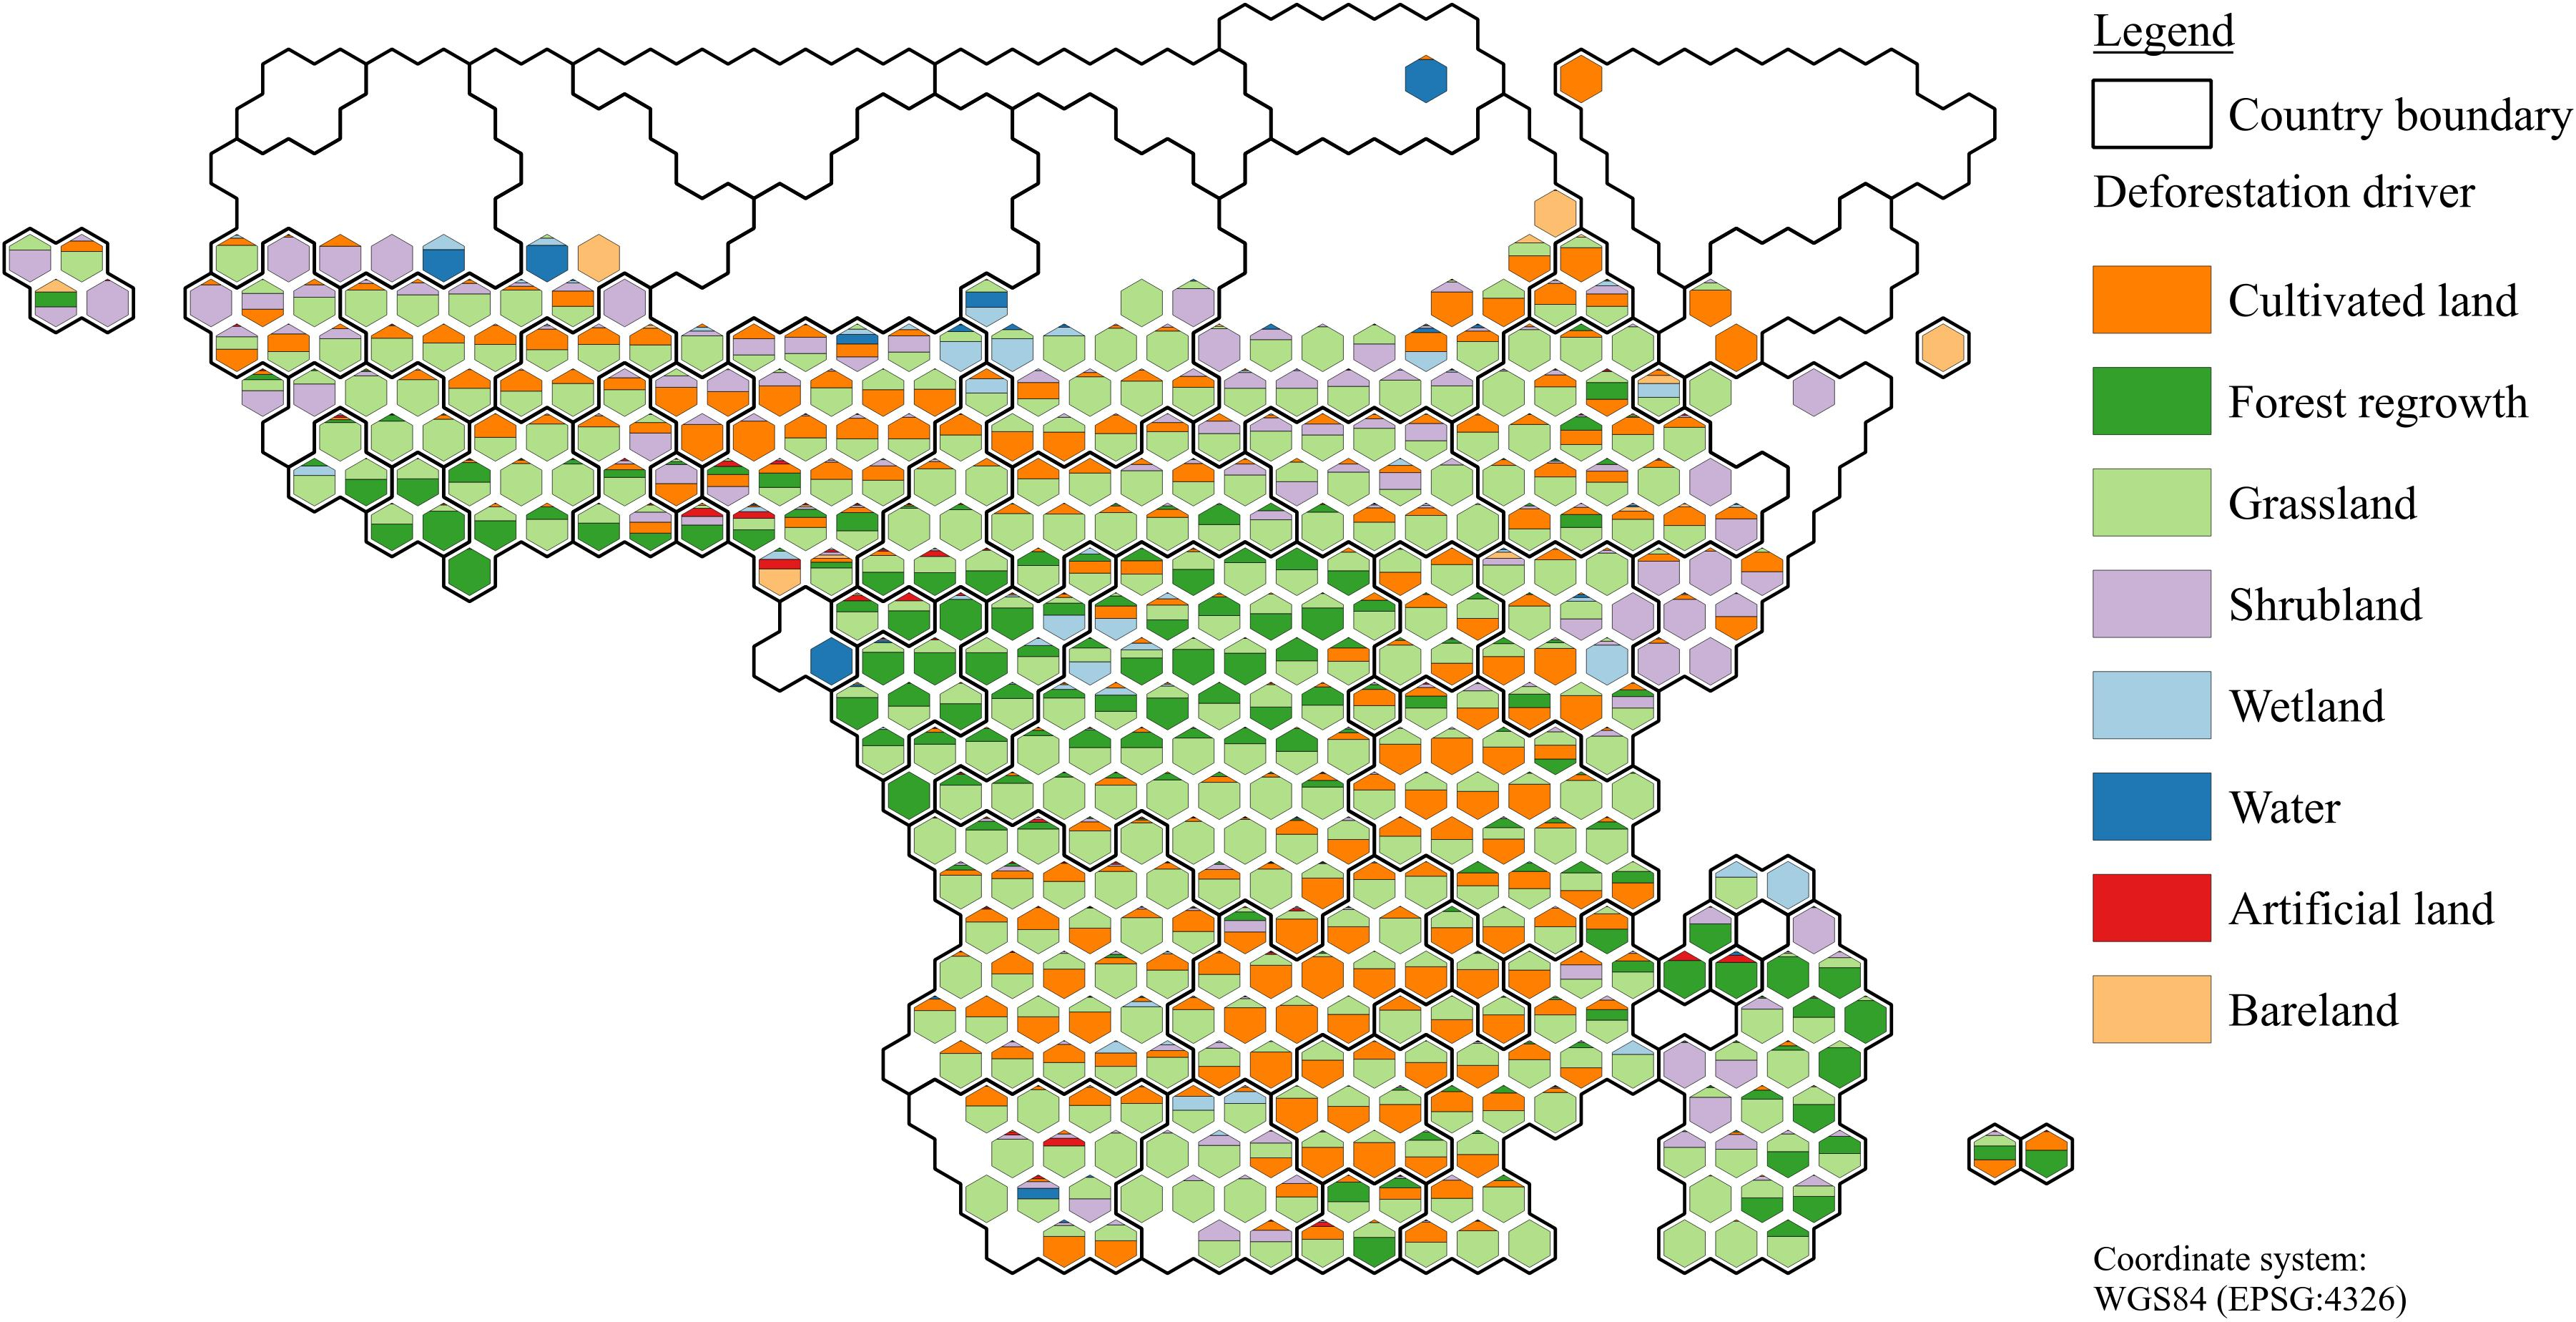
\includegraphics[scale=1]{img/africa_driver_frameless}
				\caption[Map of proximate deforestion drivers in Africa]{\textbf{Map of proximate deforestation drivers in Africa:} The map shows the distribution of proximate deforestation drivers in Africa. The different sized and colored quantities within each hexagons interior shows the relative tree cover loss by a proximate deforestation driver. Scaling of a the hexagons is only intended for improving visual appeal of \acp{PDD}.}
				\label{fig:africa_driver}
			\end{figure}

		\subsection{Accuracy assessment}
		\label{subsec:results_accuracy_assessment}
			\begin{table}[ht]
				\centering
				\caption[Accuracy assessment]{\textbf{Accuracy assessment:} We selected 200 samples by random from 10 randomly selected tiles from the three sampling stratas Latin America, Asia/Australia and Africa. Labels refer to our proximate deforestation driver classes. Reference refers to the samples we classified by visual interpretation of Google Maps high resolution imagery and predictions refer to the label the sample has in our proximate driver product. The abbreviations PAc, UAc, OvAc, Com, Om, Tot, and Kappa refer to the terms Producers-Accuracy, Users-Accuracy, Overall-Accuracy, Error of Commission, Error of Omission, row or column total, and Kappa Coefficient.}
				\label{tab:results_confusion_matrix}
				\begin{tabular}{llrrrrrrrrrrrr}
					\hline
					& & \multicolumn{9}{c}{Reference} & & & \\\cline{3-11}
					& Cls & 10 & 20 & 25 & 30 & 40 & 50 & 60 & 80 & 90 & Tot & UAc & Om \\\hline
					\multirow{9}{*}{\STAB{\rotatebox[origin=c]{90}{Prediction}}}
					& 10 & 730 & 37 & 62 & 15 & 16 & 2 & 3 & 5 & 0 & 870 & .84 & .16 \\ 
					& 20 & 41 & 744 & 56 & 189 & 31 & 12 & 0 & 15 & 4 & 1092 & .68 & .32 \\ 
					& 25 & 29 & 202 & 1155 & 172 & 22 & 10 & 5 & 11 & 4 & 1610 & .72 & .28 \\ 
					& 30 & 36 & 187 & 32 & 1466 & 73 & 21 & 0 & 17 & 0 & 1832 & .80 & .20 \\ 
					& 40 & 14 & 21 & 4 & 41 & 352 & 1 & 1 & 2 & 1 & 437 & .81 & .19 \\ 
					& 50 & 0 & 5 & 3 & 10 & 4 & 50 & 0 & 1 & 0 & 73 & .68 & .32 \\ 
					& 60 & 2 & 1 & 0 & 3 & 0 & 2 & 18 & 2 & 0 & 28 & .64 & .36 \\ 
					& 80 & 3 & 3 & 0 & 1 & 1 & 1 & 0 & 40 & 0 & 49 & .82 & .18 \\ 
					& 90 & 0 & 0 & 0 & 1 & 0 & 0 & 0 & 3 & 5 & 9 & .56 & .44 \\\hline 
					& Tot & 855 & 1200 & 1312 & 1898 & 499 & 99 & 27 & 96 & 14 & 6000 & & \\
					& PAc & .85 & .62 & .88 & .77 & .71 & .51 & .67 & .42 & .36 & Kappa & \multicolumn{2}{r}{OvAc} \\
					& Com & .15 & .38 & .12 & .23 & .29 & .49 & .33 & .58 & .64 & .69 & \multicolumn{2}{r}{.76} \\ \hline
				\end{tabular}
			\end{table}
			This section presents and discuses the accuracy assessment of the \acp{PDD} mapping, while the table \ref{tab:results_confusion_matrix} shows the results of this assessment. In total 4560 of 6000 \ac{LC} transitions are correctly classified by our approach to map the \acp{PDD} of tropical deforestation. This translates to an overall accuracy of approximately 0.76, which implies that approximately 76\% of the forest loss is correctly classified. From the 6000 samples cultivated land (10), forest (20), regrowth (25), grassland (30), shrubland (40), wetland (50), water (60), artificial surfaces (80) and bareland (90) account for 14.5\%, 18.2\%, 26.8\%, 30.5\%, 7.3\%, 1.2\%, 0.5\%, 0.8\%, and 0.1\% of the samples, respectively. This corresponds to the relative distribution of the  \acp{PDD} in table \ref{tab:proximate_driver} in the appendix \ref{ch:appendix}. 

			For the classification of tree cover loss as cultivated land the producers and users accuracy account for 0.85 and 0.84, respectively. Therefore, this class has the highest accuracy and a tendency for overestimation or underestimation is not given. For the regrowth class producers and users accuracy account for 0.88 and 0.72, respectively. This shows that regrowth is slightly overestimated, while this class was introduced by the \ac{GFC} gain layer. Section \ref{subsec:methods_gfc} explains that tree cover gains are underestimated but these underestimates are captured by the forest class. For the grassland class producers and users accuracy account for 0.77 and 0.80, respectively. In general this class show no tendencies of overestimates or underestimates. The transformation of forests to artificial surfaces is largely underestimated as the difference of producers and users accuracy, which account for 0.42 and 0.82 show. This could be attributed to our reclassification approach, which is further discussed in section \ref{sec:discussion_deforestation}. Further, the bareland class is underestimated as well, which could be attributed to the reclassification approach. The wetland class achieves an accuracy of 0.51, while the users accuracy highlights that this class is underestimated. Wetlands are highly dynamic ecosystems that change quickly its shape. Therefore, for this class it is to expect that the accuracy is lower. For water bodies the producers and users accuracy account for 0.67 and 0.68, which shows no general tendency of underestimation or overestimation. For the shrubland class the producers and users accuracy account for 0.71 and 0.81, while this shows that this class is underestimated. As beforehand mentioned the reclassification approach could lead to this effect. The reclassification tends to favor class with a higher probability, which is explained in detail in the discussion.

	\section{Carbon loss}
	\label{sec:results_carbon_loss}
		At a global scale the removal of biomass accounts for a total carbon loss of approximately 6757 Mt C between 2001-2010 (table \ref{tab:soce_tab}). \citet{Achard2014} estimates that the total carbon loss from tropical deforestation is between 6020-12370 Mt C for the same period. The total carbon loss by \ac{SOC} change is in the 478-688 Mt C range, if we assume that all deforestation occurs within primary forest (SC$_1$). For the second scenario (SC$_2$) we estimated a carbon loss range of 226-378 Mt C. The carbon loss by \ac{SOC} change would add 3.3-10.2\% Mt C to the total carbon loss of tropical deforestation.

		In Latin America the total carbon loss accounts for approximately 3198 Mt C for the removal of \ac{AGB} by tropical tree cover loss (table \ref{tab:soce_tab}). \citet{Achard2014} estimates that the total carbon loss is between 3226-6497 Mt C for the period 2001-2010, while \citet{Sy2015} measures a carbon loss range of 5959-6961 Mt C between 1990-2005. The comparison with our estimates shows that our results do not largely differ from the literature, despite the differences in applied methodology. By applying the first scenario carbon losses by \ac{SOC} change accounted for 259 ($\pm$ 44) Mt C, while for the second scenario the carbon losses account for 165 ($\pm$ 44) Mt C, respectively. Therefore, \ac{SOC} change adds between 3.8-9.5\% Mt C to the total carbon loss from tropical deforestation.

		For Asia/Australia the removal of \ac{AGB} accounts for a total carbon loss of approximately 2063 Mt C (table \ref{tab:soce_tab}), while \citet{Achard2014} estimates a carbon loss between 2355-3670 Mt C for the period 2001-2010. If we assume that the entire deforestation occurred in primary forest the carbon loss by \ac{SOC} change would account for roughly 220 ($\pm$ 43) Mt C, while carbon loss would account for 76 ($\pm$ 16) Mt C if we distinguish between deforestation of primary and secondary forest. Carbon loss by \ac{SOC} change adds 2.9-12.7\% Mt C to the total carbon loss in Asia/Australia.

		In Africa the total carbon loss account for approximately 1496 Mt C. \citet{Achard2014} measures a carbon loss range of 430-2220 Mt C for the period 2001-2010. For the first scenario carbon loss by \ac{SOC} change accounted for 104 ($\pm$ 18) Mt C, while carbon loss accounts for 61 ($\pm$ 16) Mt C in the second scenario. This would add approximately 3-8.2\% Mt C to the total carbon loss.
		\begin{table}[ht]
			\centering
			\caption[Carbon loss]{\textbf{Carbon loss:} The columns SC$_1$ and SC$_2$ refer to soil organic carbon loss scenarios (soil organic carbon change coefficients depend on forest type): SC$_1$ assumes that all deforestation occurs in primary forest, and SC$_2$ uses a additional stratum to distinct between primary and secondary forest. Biomass refers to carbon loss by biomass removal (aboveground and below-ground biomass). The unit of all measurements is Mt C and standard errors are given in brackets if available.}
			\label{tab:soce_tab}
			\begin{tabular}{lccrc}
				\hline
				\multirow{2}{*}{Region}& \multicolumn{2}{c}{Soil} && \multirow{2}{*}{Biomass} \\\cline{2-3}
				& SC$_1$ & SC$_2$ && \\\hline
				Latin America & 259 ($\pm$ 44) & 165 ($\pm$ 44) && 3198\\
				Asia/Australia & 220 ($\pm$ 43) & 76 ($\pm$ 16) && 2063\\
				Africa & 104 ($\pm$ 18) & 61 ($\pm$ 16) && 1496\\
				Global & 583 ($\pm$ 105) & 302 ($\pm$ 76) && 6757\\\hline
			\end{tabular}
		\end{table}

	\section{Ecosystem service values}
		At a global scale between 2001 and 2010, a tree cover loss of approximately 772 thousand km$^2$ accounts for an \ac{ESV} gross loss of 414.1 (Co), 405.2 (Dg), and 101.1 (Wb) billion dollars per year as table \ref{tab:esv_results} shows. By applying the \ac{ESV} unit value for tropical forest from \citet{Costanza2014} the expansion of cropland and pastures accounts for a gross loss of approximately 95.3 and 128 billion dollars per year, respectively. The transition of forest cover to artificial surfaces and regrowth dynamics accounts for a gross loss of 2.3 and 124 billion dollars per year. If we consider the monetary value of tropical forest from \citet{Siikamaki2015} cropland, grassland, artificial surfaces, and regrowth dynamics accounted for a gross loss of approximately 23.2, 46.7, 0.5, and 30.2 billion dollars per year.

		The gross gain in \ac{ESV} from \ac{LC} transitions of tropical forest cover accounts for 350.6, 208.7, and 31.0 billion dollars per year for the three datasets. By using the unit values of the first dataset cropland, pastures, artificial surfaces, and regrowth dynamics accounted for a gross gain of 98.5, 120.6, 2.4, and 124.1 billion dollars per year. If we consider \citet{Groot2012} unit values grassland and regrowth account for a gain of 83 and 121 billion dollars per year, respectively, while regrowth dynamics account for a gross gain of approximately 31 billion dollars for the last dataset.

		At a global scale, the net loss of tropical forest change accounts for 63.5, 196, and 70.1 billion dollars per year for the three datasets Co, Dg, and Wb. The greatest net loss can be observed by applying the \citet{Groot2012} unit values, which could be attributed to the limited number of \acp{PDD} classes covered by an \ac{ESV} unit value. The relatively small net loss by using the unit values of the first dataset can be explained on the fact that approximately a fifth of the global tree cover is lost through the expansion of cropland. \citet{Costanza2014} estimates 5567 Int'I\$ y$^{-1}$ as the \ac{ESV} for cropland, which is 1.03 times greater than the \ac{ESV} of tropical forest. Further, roughly a quarter of the tropical forest is exposed to regrowth dynamics, which uses the equivalent \ac{ESV} as tropical tree cover. Therefore, approximately half of the tropical forest cover is replaced by \ac{LC} types, which have a greater or equal \ac{ESV} than the \ac{ESV} of tropical forest.

		For the 2000-2012 time period, \citet{Song2018} assesses that deforestation accounts for an \ac{ESV} net loss of 550.7 billion dollars per year. The difference to our \ac{ESV} net loss estimate can be attributed to discrepancies in \ac{LC} change area assessment, forest definition, and temporal resolution. \citet{Song2018} quantified the \ac{ESV} gross loss from tree cover losses within the entire canopy density interval. Further, the study considered only \ac{ESV} gain from forest regrowth, while other \ac{LC} change types are not included.
		\begin{table}[ht]
			\centering
			\caption[Ecosystem service value balance]{\textbf{Ecosystem service value balance:} The dataset column refers to the three global ecosystem service value datasets by \citet{Costanza2014} (Co), \citet{Groot2012} (Dg), and \citet{Siikamaki2015} (Wb). Loss refers to the monetary value of tropical forest deforested by the following aggregated anthropogenic proximate deforestation drivers: cropland, grassland, regrowth, shrubland, artificial surfaces, and bareland. Gain is the monetary value of the land cover transition and balance is difference of gain and loss. Monetary unit of the ecosystem service values is 10$^{9}$ 2007 Int'I\$ y$^{-1}$ (billion international dollars 2007 per year).}
			\label{tab:esv_results}
			\begin{tabular}{lrrrr}
				\hline
				Dataset & Latin America & Asia/Australia & Africa & Global\\
				\hline
				Co$_{loss}$ & 208.3 & 111.6 & 94.2 & 414.1 \\
				Co$_{gain}$ & 161.0 & 109.1 & 80.6 & 350.6 \\
				Co$_{balance}$ & -47.3 & -2.5 & -13.6 & -63.5\\
				Dg$_{loss}$ & 204.0 & 109.1 & 92.1 & 405.2\\
				Dg$_{gain}$ & 82.5 & 83.1 & 43.1 & 208.7\\
				Dg$_{balance}$ & -121.5 & -26.0 & -49.0 & -196.5\\
				Wb$_{loss}$ & 51.0 & 27.2 & 22.9 & 101.1\\
				Wb$_{gain}$ & 7.3 & 19.4 & 4.3 & 31.0 \\
				Wb$_{balance}$ & -43.7 & -7.8 & -18.6 & -70.1 \\
				\hline
			\end{tabular}
		\end{table}

		In Latin America a forest loss of approximately 396 thousand km$^2$ accounts for a gross loss of 208.3 (Co), 204 (Dg), or 51 (Wb) billion 2007 Int'I\$ y$^{-1}$ (table \ref{tab:esv_results}). By applying the \citet{Costanza2014} unit value the transition of tree cover to cropland accounts for a gross loss of 51 billion Int'I\$ y$^{-1}$, while transitions to pastures accounted for a gross loss of approximately 126 billion dollars per year. Deforestation for the expansion of artificial and bareland surfaces accounted for a gross loss of 1 billion Int'I\$ y$^{-1}$, respectively, while regrowth dynamics convert to a gross loss of 30 billion dollars. By applying the unit value of tropical forest from \citet{Siikamaki2015} the transitions to cropland and pastures cost 12.6 and 30.6 billion dollars. Further, urbanization and bareland transitions accounted for a gross loss of 0.3 billion dollars per year, while regrowth dynamics accounted for 7.5 billion international dollars per year. The gross loss estimate variability between both unit value datasets is related to the valuation difference of tropical forest. \citet{Costanza2014} unit value for the tropical forest is approximately 4 times greater than \citet{Siikamaki2015}.

		We estimated a gross gain of 161 billion dollars per year for the Co dataset. The table \ref{tab:esv_mapping} in section \ref{subsec:methods_esv} suggests that we calculated the gross gain from \ac{LC} transitions to cropland, grassland, artificial surfaces, and regrowth, which accounted for a gross gain of 53.4, 76.6, 1, and 30.6 billion dollars per year. By applying the \citet{Groot2012} \ac{ESV} estimates the gross gain from \ac{LC} transitions accounted for 82.5 billion dollars per year. This converts to a gross gain from grassland and regrowth transitions of approximately 52.8 and 29.9 billion dollars. The last dataset we tested enabled us to compute only the gross gain from tree cover regrowth which accounts for a monetary gain of 7.3 billion dollars per year.

		In Latin America, the net loss accounts for 47.3, 121.5, and 43.7 billion dollars for Co, Dg, and Wb. The highest net loss can be recognized by applying the Dg unit values, but this relates to the limited number of \ac{LC} transitions covered by a valuation.

		In Asia/Australia a tree cover loss of approximately 230 thousand km$^2$ accounts for a gross loss of 111.6 (Co), 109.1 (Dg), or 27.2 (Wb) billion dollars per year as table \ref{tab:esv_results} shows. By applying the unit value of the first dataset the transitions to cultivated and grassland accounts for a gross loss of 19.8 and 9.8 billion dollars per year, respectively. Further, the expansion of artificial surfaces accounted for a gross loss of 0.5 billion dollars, while the regrowth dynamics accounted for a gross loss of approximately 75.7 billion dollars per year. By applying the monetary \ac{ESV} unit value for tropical forest from \citet{Siikamaki2015} cropland and pastures accounted for a gross loss of 4.8 and 2.4 billion dollars per year, respectively. The transition of forest cover to artificial surfaces account for 0.2 billion dollars, while regrowth accounts for 18.4 billion dollars.

		In regards to \ac{ESV} gain dynamics and by applying the first dataset cropland and pastures account for a monetary gross gain of 20.5 and 6.8 billion dollars per year, respectively. Further \ac{LC} transitions to regrowth and artificial surfaces accounted for a gross gain of 75.7 and 0.5 billion dollars. By considering \citet{Groot2012} estimates grassland and regrowth accounted for a gross gain of approximately 4.6 and 74 billion dollars per year, respectively. By applying the last dataset in table \ref{tab:esv_results} regrowth accounts for a gain of 19.4 billion dollars per year.

		In regards to the net \ac{ESV} balance in Asia/Australia, the three datasets accounted for a net loss of 2.5, 26, and 7.8 billion dollars per year. The low net losses can be explained by the high quantities of regrowth. In Asia/Australia the large quantities of regrowth could be the establishment of plantations or the rotational cycle as a management practice for existing plantations.

		For Africa, the table \ref{tab:esv_results} shows that a tree cover loss of approximately 177 km$^2$ accounts for a gross \ac{ESV} loss of 94.2 (Co), 92.1 (Dg), and 22.9 (Wb) billion dollars per year for the three datasets. For the first dataset tree cover losses by cultivated and grassland expansion accounts for a gross loss of 23.7 and 51.5 billion dollars, respectively, while the expansion of artificial surfaces accounts for 0.7 billion dollars. In Africa, regrowth dynamics are responsible for a gross loss of approximately 17.7 billion dollars per year. By applying the monetary value for the tropical forest of \citet{Siikamaki2015} cropland and pasture expansion accounted for a gross loss of 5.8 and 12.7 billion dollars per year, respectively. The transition to artificial surfaces accounted for 0.2 billion dollars, while regrowth dynamics accounted for a gross loss of 4.3 billion dollars. 

		The monetary gross gain by \ac{LC} transitions accounts for 80.6, 43.1, and 4.3 billion dollars per year. For the Co dataset the forest transition to cropland, pastures, artificial surfaces, and regrowth dynamics accounts for a gross gain of 24.6, 37.2, 0.8, and 17.7 billion dollars. By applying the second dataset grassland and regrowth dynamics accounts for a gross gain of 25.6 and 17.4 billion dollars, respectively, while the last dataset estimates a gross gain of approximately 4.3 billion dollars for regrowth dynamics. In Africa the net loss accounts for 13.6 (Co), 49 (Dg), and 18.6 (Wb) billion dollars.

		The highest \ac{ESV} gross loss can be observed in Latin America followed by Asia/Australia and Africa. This gross loss dynamic is mainly attributed to the large area deforested in Latin America. If we normalize the Co \ac{ESV} gross gain by dividing through the deforestation per continent the normalized gross gain accounts for 414, 553, and 462 thousand Int'I\$ y$^{-1}$ km$^{-2}$ for Latin America, Asia/Australia, and Africa. Therefore, the highest \ac{ESV} gross gain per deforested km$^2$ of tropical forest can be observed in Asia/Australia followed by Africa, while Latin America has the lowest \ac{ESV} gain per km$^2$. This can be attributed to the large number of regrowth dynamics in Asia/Australia. In Africa, the \ac{ESV} gross gain is mainly caused by a large number of agricultural transitions and regrowth dynamics. The \ac{ESV} net losses are the smallest in Asia/Australia followed by Africa, while Latin America has the greatest net loss. Differences in \ac{ESV} estimates between the datasets of \citet{Costanza2014}, \citet{Groot2012}, and \citet{Siikamaki2015} are mainly attributed to the completeness of biomes represented and the valuation.